%Talk given at IIT's Computational Math and Stats Seminar 2019 August
\documentclass[10pt,compress,xcolor={usenames,dvipsnames},aspectratio=169]{beamer}
%\documentclass[xcolor={usenames,dvipsnames},aspectratio=169]{beamer} %slides and 
%notes
\usepackage{amsmath,datetime,
	mathtools,
	bbm,
	%mathabx,
	array,
	booktabs,
	xspace,
	calc,
	colortbl,
	scrextend,
 	graphicx}
\addtokomafont{labelinglabel}{\itshape\textcolor{IITred!80!IITgray}}
\usepackage[usenames]{xcolor}
\usepackage[giveninits=false,backend=biber,style=nature, maxcitenames =10, mincitenames=9]{biblatex}
\addbibresource{FJHown23.bib}
\addbibresource{FJH23tweak.bib}
\usepackage{newpxtext}
\usepackage[euler-digits,euler-hat-accent]{eulervm}
\usepackage{media9}
\usepackage[autolinebreaks]{mcode}

\usetheme{FJHSlimNoFoot169}
\setlength{\parskip}{2ex}
\setlength{\arraycolsep}{0.5ex}

\newcommand{\contradiction}{%
  \ensuremath{{\Longrightarrow\mspace{-2mu}\Longleftarrow}}%
}

\DeclareMathOperator{\sol}{SOL}
\DeclareMathOperator{\app}{APP}
\DeclareMathOperator{\alg}{ALG}
\DeclareMathOperator{\ERR}{ERR}
\DeclareMathOperator{\COST}{COST}
\newcommand{\dataN}{\bigl(\hf(\vk_i)\bigr)_{i=1}^n}
\newcommand{\dataNj}{\bigl(\hf(\vk_i)\bigr)_{i=1}^{n_j}}
\newcommand{\dataNjd}{\bigl(\hf(\vk_i)\bigr)_{i=1}^{n_{j^\dagger}}}
\newcommand{\ERRN}{\ERR\bigl(\dataN,n\bigr)}

\newcommand{\Sapp}{S_{\textup{app}}} 
\newcommand{\LambdaStd}{\Lambda^{\textup{std}}}
\newcommand{\LambdaSer}{\Lambda^{\textup{ser}}}
\newcommand{\LambdaAll}{\Lambda^{\textup{all}}}
%\DeclareMathOperator{\spann}{span}
%\DeclareMathOperator{\app}{app}

\providecommand{\HickernellFJ}{H.}


\iffalse
The Challenges of Approximating Functions of Many Variables
Fred J. Hickernell, Department of Applied Mathematics, Illinois Institute of Technology, Chicago, IL

Function approximation is relatively simple compared to many other continuous numerical problems, such as solving (stochastic and/or partial) differential equations. Interpolation is often used in the case of noiseless data, and regression can handle the case of noisy data.  For functions of one variable, collecting sufficient data is often straightforward, but for functions of many variables the function must satisfy some simplifying structure for approximation to be successful.  The problem is even more difficult when functions values are costly, such as when they are generated by some complex computer simulation.  This talk highlights some of the challenges of approximating functions of many variables and the strategies for overcoming these challenges.

\fi

\renewcommand{\OffTitleLength}{-10ex}
\setlength{\FJHThankYouMessageOffset}{-8ex}
\title{The Challenges of Approximating Functions of Many Variables}
\author[]{Fred J. Hickernell}
\institute{Department of Applied Mathematics \\
	Center for Interdisciplinary Scientific Computation \\  Illinois Institute of Technology \\
	\href{mailto:hickernell@iit.edu}{\url{hickernell@iit.edu}} \quad
	\href{http://mypages.iit.edu/~hickernell}{\url{mypages.iit.edu/~hickernell}}}

\thanksnote{Joint work with Yuhan Ding, Peter Kritzer, and Simon Mak \\
	This work partially supported by  NSF-DMS-1522687 and NSF-DMS-1638521 (SAMSI) 
}
\event{Computational Mathematics and Statistics Seminar}
\date[]{August 30, 2019}

\input FJHDef.tex


%Abstract:  When

\newlength{\figwidth}
\setlength{\figwidth}{0.25\textwidth}

\newlength{\figwidthSmall}
\setlength{\figwidthSmall}{0.2\textwidth}

\newcommand{\financePict}{\href{http://i2.cdn.turner.com/money/dam/assets/130611131918-chicago-board-options-exchange-1024x576.jpg}{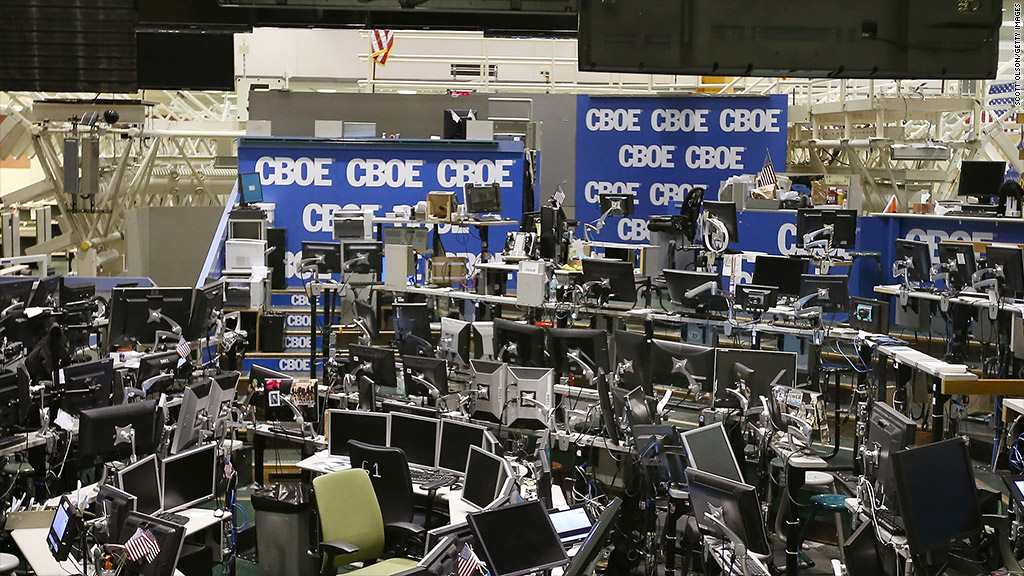
\includegraphics[width
		= 3cm]{ProgramsImages/130611131918-chicago-board-options-exchange-1024x576.jpg}}}
	
	\newcommand{\scoop}[1]{\parbox{#1}{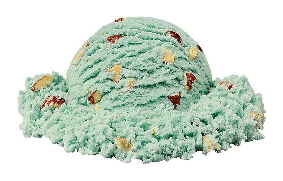
\includegraphics[width=#1]{IceCreamScoop.eps}}\xspace}
	\newcommand{\smallscoop}{\scoop{1cm}}
	\newcommand{\medscoop}{\scoop{1.8cm}}
	\newcommand{\largescoop}{\scoop{3cm}}
	\newcommand{\ICcone}[1]{\parbox{#1}{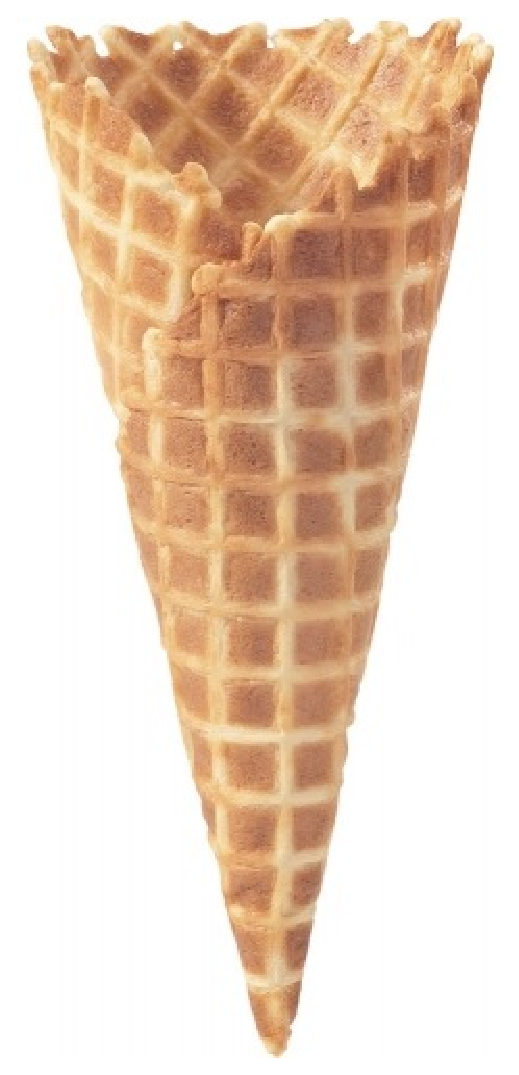
\includegraphics[width=#1,angle=270]{MediumWaffleCone.eps}}\xspace}
	\newcommand{\medcone}{\ICcone{1.2cm}}
	\newcommand{\largercone}{\parbox{2.2cm}{\vspace*{-0.2cm}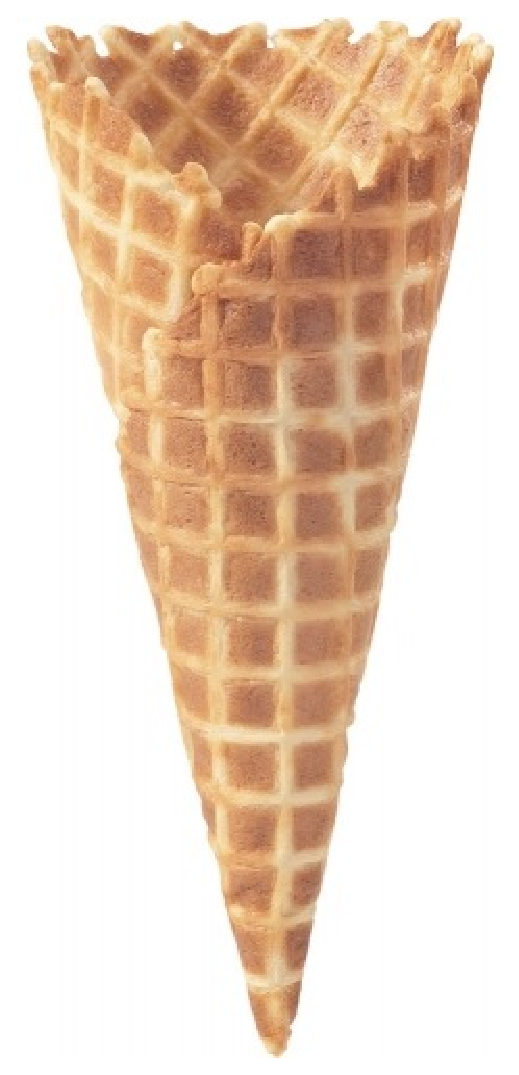
\includegraphics[width=1cm,angle=270]{MediumWaffleCone.eps}}\xspace}
	\newcommand{\largecone}{\ICcone{1.8cm}}
	\newcommand{\smallcone}{\parbox{1.1cm}{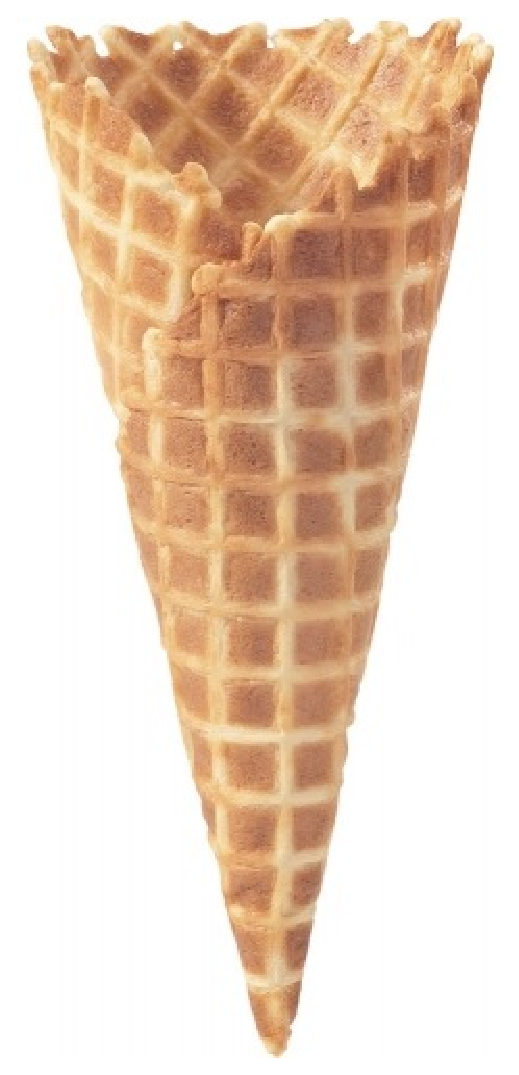
\includegraphics[width=0.5cm,angle=270]{MediumWaffleCone.eps}}\xspace}

	


\begin{document}
\everymath{\displaystyle}
\frame{\titlepage}



\section{Introduction}

\begin{frame}[label = high]{Highlights}

\vspace{-8ex}

\alert{Goal:} Construct $\alg$  such that given a \alert{black box} providing information about $f: \Omega \subset \reals^{\alert{d}} \to \reals$
\begin{equation*}
    \norm[\cg]{f - \alg(f,\varepsilon)} \le \varepsilon \qquad \forall \varepsilon > 0, \; f \in \ch \subseteq \cf \text{ (Banach space)}
\end{equation*}

\begin{itemize}
    \item \alert{Impossible} for infinite dimensional Banach space $\ch = \cf$, so what is $\ch$?
    
    \item \alert{Smoothness} assumed by $\cf$ speeds up $\alg$, not surprising
    
    \item Smoothness alone cannot save from the \alert{curse of dimensionality}, but a low effective-dimension structure can
    
    \item Choosing $\ch$ to be a \alert{cone}\smallcone, rather than a ball\smallscoop, paves the way for \alert{adaptive} algorithms
    
    \item Interesting \alert{design} (where to sample) problems remain
\end{itemize}
    
\end{frame}


\begin{frame}{Problem}

\vspace{-5ex}

\begin{itemize}[]
    \item  Input
    \begin{addmargin}{3ex}
    \begin{labeling}{Error Tolerance}
       \item[Black box] providing \alert{noiseless} information about $f:\Omega \subseteq \reals^d \to \reals$
    \only<1-2>{ \\ e.g., function values or series coefficients,} \alert{costing} $\$(f)$ each
       \only<3->{\\ \alert<3>{$f \in \cf$, definition of $\norm[\cf]{\cdot}$ enshrines smoothness assumptions}}
        
        \item[Error tolerance] $\varepsilon$
     
    \end{labeling}
    \end{addmargin}
    \vspace{1ex}
    
    \item Output $\alg(f,\varepsilon)$ \only<1>{(as a surrogate, for solving PDEs, for uncertainty quantification) }that is
    \begin{addmargin}{3ex}
    \begin{labeling}{Accurate}
        \item[Cheap] to evaluate and manipulate
        
        \item[Accurate] $\norm[\cg]{f - \alg(f,\varepsilon)} \le \varepsilon \qquad \forall \varepsilon > 0\uncover<3->{, \ \alert<3>{f \in \ch \subset \cf}}$%
        \uncover<3->{\alert<3>{, provably}}
        
        \item[Efficient] to construct

    \end{labeling}
    \end{addmargin}
    \vspace{1ex}

	\item<2-> Approximation  with fixed computation budget: $\app(f,n) = \sum_{i=1}^n L_i(f) g_{i,n}$
	\setbeamertemplate{itemize items}[triangle]
	\begin{itemize}
	    \item $L_1(f), L_2(f), \ldots$ is input function information% 
	    \only<2>{, e.g., function values or series coefficients}
	    \item $\vg_n = (g_{1,n}, \ldots, g_{n,n}) \in \cg^n$ \quad \alert{cardinal functions}
	    \item $ \alert{\COST(f,n)} = \Order(n \$(f) + \COST( \vg_n))$
	\end{itemize}
    \vspace{1ex}
	
	\item<2-> Algorithm $\alg(f,\varepsilon) = \app(f,n^*(f,\varepsilon))$ satisfying  
	$\norm[\cg]{f -  \app(f,n^*(f,\varepsilon))} \le \varepsilon \ \  \forall \varepsilon > 0 \uncover<3->{,\ \alert<3>{f \in \ch \subset \cf}}$
	
	\setbeamertemplate{itemize items}[triangle]
		\begin{itemize}
	    \item $ \alert{\COST(f,\varepsilon)} = \COST(f,n^*(f,\varepsilon)) + \text{ cost to determine } n^*(f,\varepsilon)$
	\end{itemize}


\end{itemize}

\end{frame}

%%%%%%%%%%%%%%%%%%%%%%%%%%%%%%%%%%%%%%%%%%%%%%%%%%%%%%%%%%%%%%%%%%%%
\section{Solvability}
%%%%%%%%%%%%%%%%%%%%%%%%%%%%%%%%%%%%%%%%%%%%%%%%%%%%%%%%%%%%%%%%%%%%

\begin{frame}{Impossible for All $f$ in Infinite Dimensional $\cf$}
\vspace{-5ex}
\[
\norm[\cg]{f - \alg(f,\varepsilon)} \le \varepsilon \quad \forall f \in \ch \alert{\subset} \cf
\]
\alert{Proof by contradiction}

\vspace{-3ex}
\begin{itemize}
    \item Suppose $\ch = \cf$
    
    \item Fix $\varepsilon > 0$
    
    \item Let $L_1, \ldots, L_n$ be the linear information used to construct $\alg(\alert{0},\varepsilon)$
    
    \item Choose \alert{nonzero fooling function} $f \in \cf$, such that $L_1(f) = \cdots = L_n(f) = 0$
    
    \item $\alg(\pm cf,\varepsilon) = \alg(0,\varepsilon)$ for all $c > 0$
    
    \item For all $c > 0$
    \begin{align*}
        \varepsilon & \ge \max\bigl(\norm[\cg]{cf - \alg(cf,\varepsilon)}, \norm[\cg]{-cf - \alg(-cf,\varepsilon)} \bigr) \\
        & \ge \frac 12 \bigl(\norm[\cg]{cf - \alg(cf,\varepsilon)} + \norm[\cg]{-cf - \alg(-cf,\varepsilon)} \bigr) \\
        & \ge \frac 12 \bigl(\norm[\cg]{cf - \alg(0,\varepsilon)} + \norm[\cg]{cf + \alg(0,\varepsilon)} \bigr) \\
        & \ge  c \norm[\cg]{f} \qquad \contradiction
    \end{align*}
    
\end{itemize}

\end{frame}

%%%%%%%%%%%%%%%%%%%%%%%%%%%%%%%%%%%%%%%%%%%%%%%%%%%%%%%%%%%%%%%%%%%%
\section{Smoothness}
%%%%%%%%%%%%%%%%%%%%%%%%%%%%%%%%%%%%%%%%%%%%%%%%%%%%%%%%%%%%%%%%%%%%

\begin{frame}<1>[label = smoothness]{Smoothness Makes Algorithm Less Expensive}
\vspace{-3ex}
For \alert{$d = 1$}, let $\{u_0, u_1, \ldots\}$ be an orthogonal (polynomial) basis for $\cf$ and $\cg$

\vspace{-6ex}
\begin{gather*}
    \cf := \left \{ f = \sum_{k=0}^\infty \hf(k) u_k  : \norm[\cf]{f} : = \norm[2]{\left(\frac{\hf(k)}{\lambda_k} \right)_{k=0}^\infty } < \infty \right \}, \qquad \lambda_0 \ge  \lambda_1 \ge \cdots > 0 \\
   \cg := \left \{ g = \sum_{k=0}^\infty \hg(k) u_k  : \norm[\cg]{g} : = \norm[2]{\bigl(\hg(k) \bigr)_{k=0}^\infty } < \infty \right \}, \qquad \app(f,n) = \sum_{k=0}^{n-1} \hf(k) u_{k} 
   \uncover<2->{\\
   \norm[\cg]{f - \app(f,n)} 
   = \norm[2]{\bigl(\hf(k) \bigr)_{k=n}^\infty } 
   = \norm[2]{\left(\frac{\lambda_k \, \hf(k)}{\lambda_k} \right)_{k=n}^\infty} \underbrace{\le}_{\text{tight}} \norm[\cf]{f} \lambda_{n} \alert{\overset{?}{\le}} \varepsilon, \quad \alert{\text{require } \lambda_n \downarrow 0}}
\end{gather*}

\uncover<3->{
\vspace{-3ex}
By choosing $\ch = \cb_R := \{ f \in \cf : \norm[\cf]{f} \le R\}$, we can define our \alert{algorithm}
\begin{gather*}
    \alg(f,\varepsilon) 
    = \app(f,n^*)\ \ \&  \ \ n^* = \min\{n : \lambda_{n} \le \varepsilon/R\} \quad \implies \quad 
    \norm[\cg]{f - \alg(f,\varepsilon)} \le \varepsilon \quad \forall f \in \cb_R\\ 
    \lambda_n = \Order(n^{-1/p}) \implies \COST(\cb_R,\varepsilon) = \Order(R^p\varepsilon^{-p})
\end{gather*}
\vspace{-7ex}
\begin{itemize}
    \item<4-> $\alg$ has \alert{optimal} cost among all successful algorithms using Fourier coefficients \\
    (look at the cost of approximating the zero function)
    \item<5-> Similar results for algorithms based on \alert{function values}, but need to choose the \alert{design} carefully
\end{itemize}
}
    
\end{frame}

\begin{frame}{Bases for Function Approximation}
\vspace{-3ex}
	\begin{tabular}{>{\centering}m{0.18\textwidth}>{\centering}m{0.18\textwidth}>{\centering}m{0.18\textwidth}>{\centering}m{0.18\textwidth}>{\centering}m{0.18\textwidth}}
		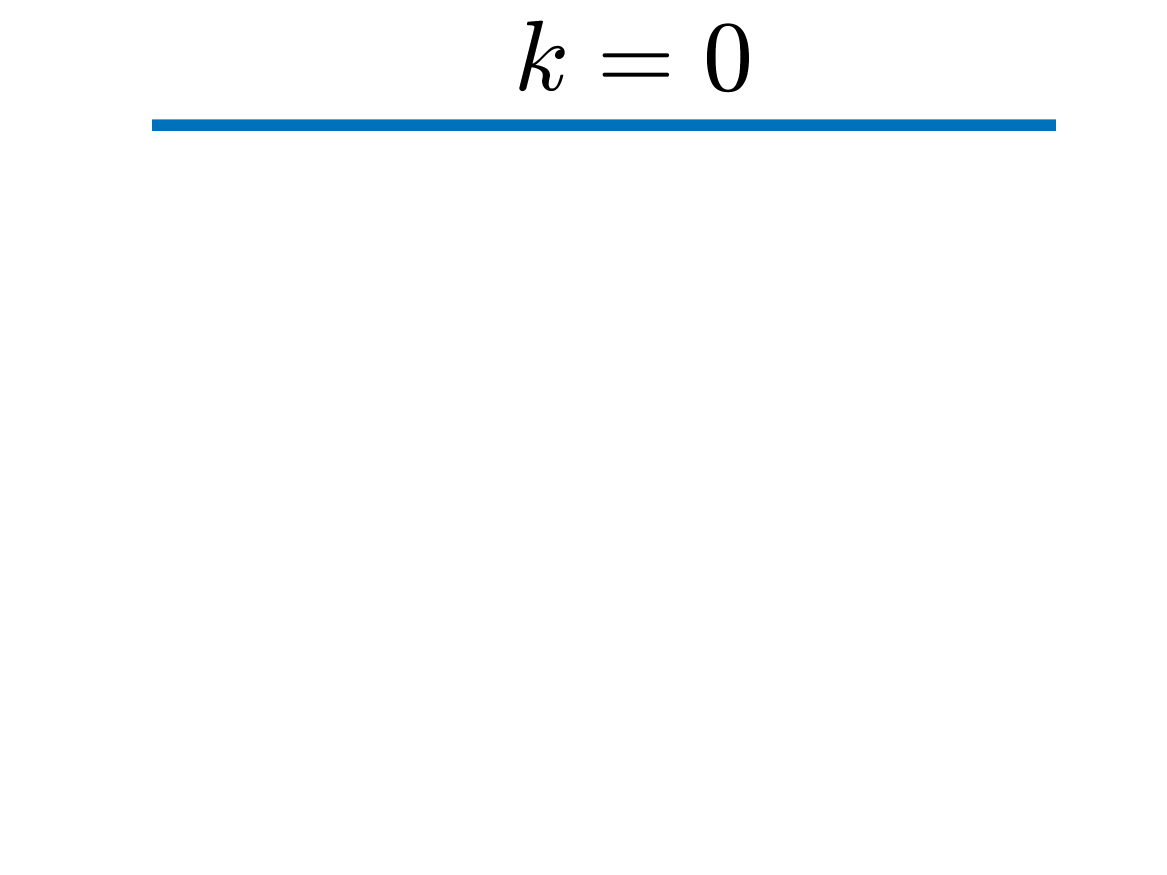
\includegraphics[width =0.18\textwidth]{ProgramsImages/Legendre_Degree_0_1D_k.png}  &
		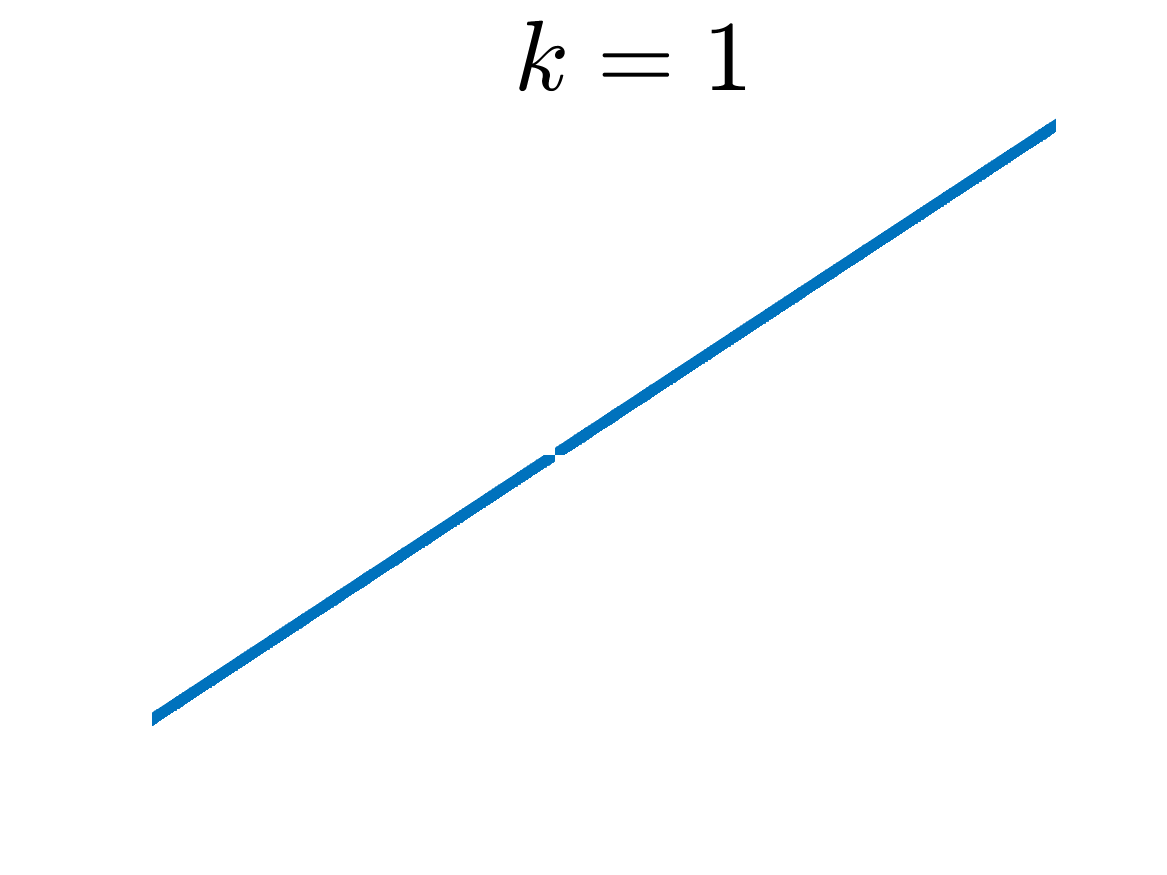
\includegraphics[width =0.18\textwidth]{ProgramsImages/Legendre_Degree_1_1D_k.png}  &
		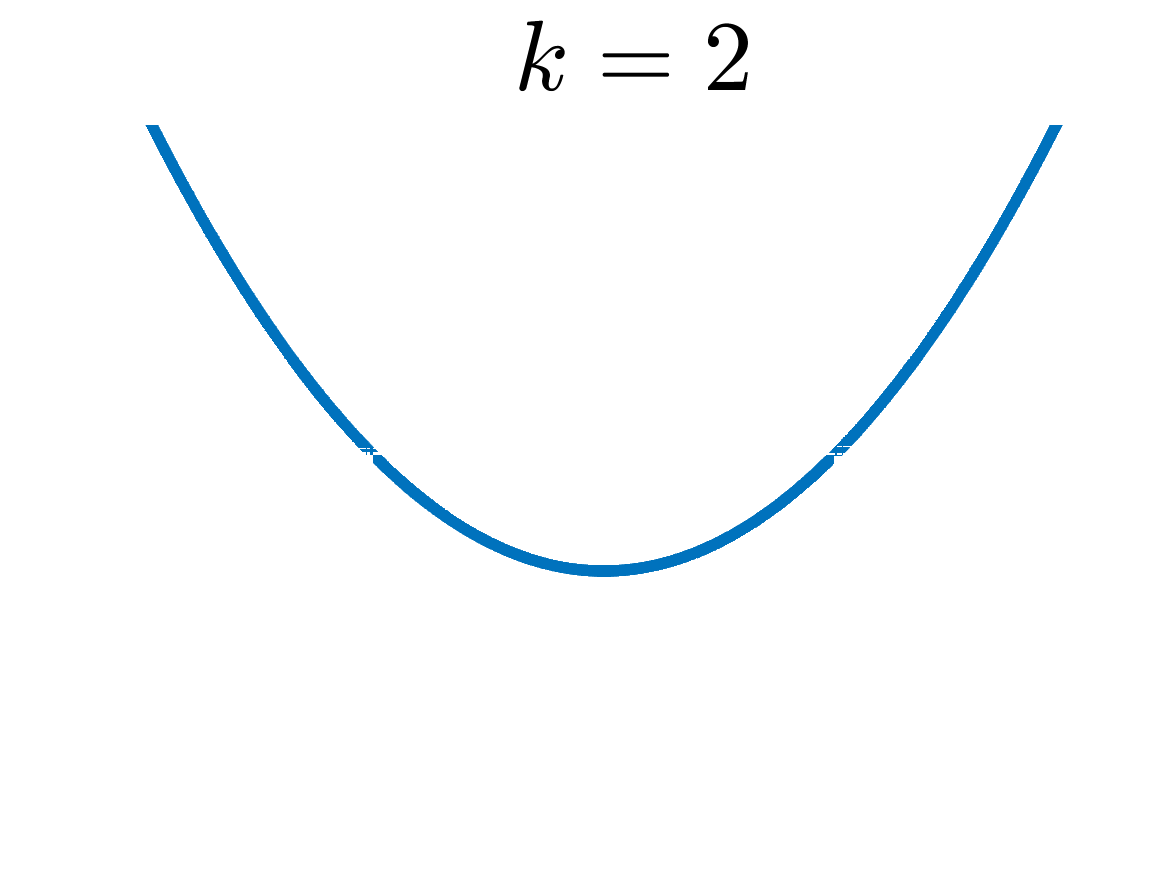
\includegraphics[width =0.18\textwidth]{ProgramsImages/Legendre_Degree_2_1D_k.png}  &
		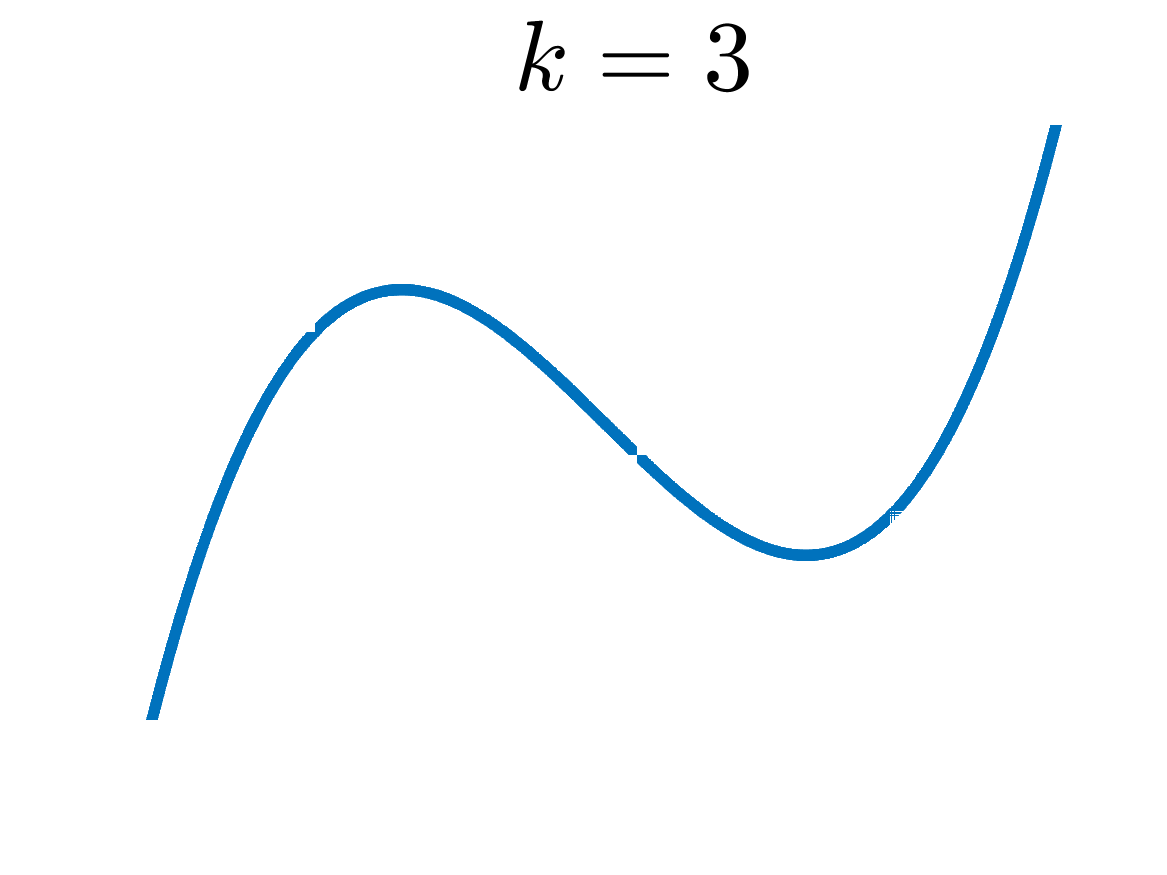
\includegraphics[width =0.18\textwidth]{ProgramsImages/Legendre_Degree_3_1D_k.png}  &
		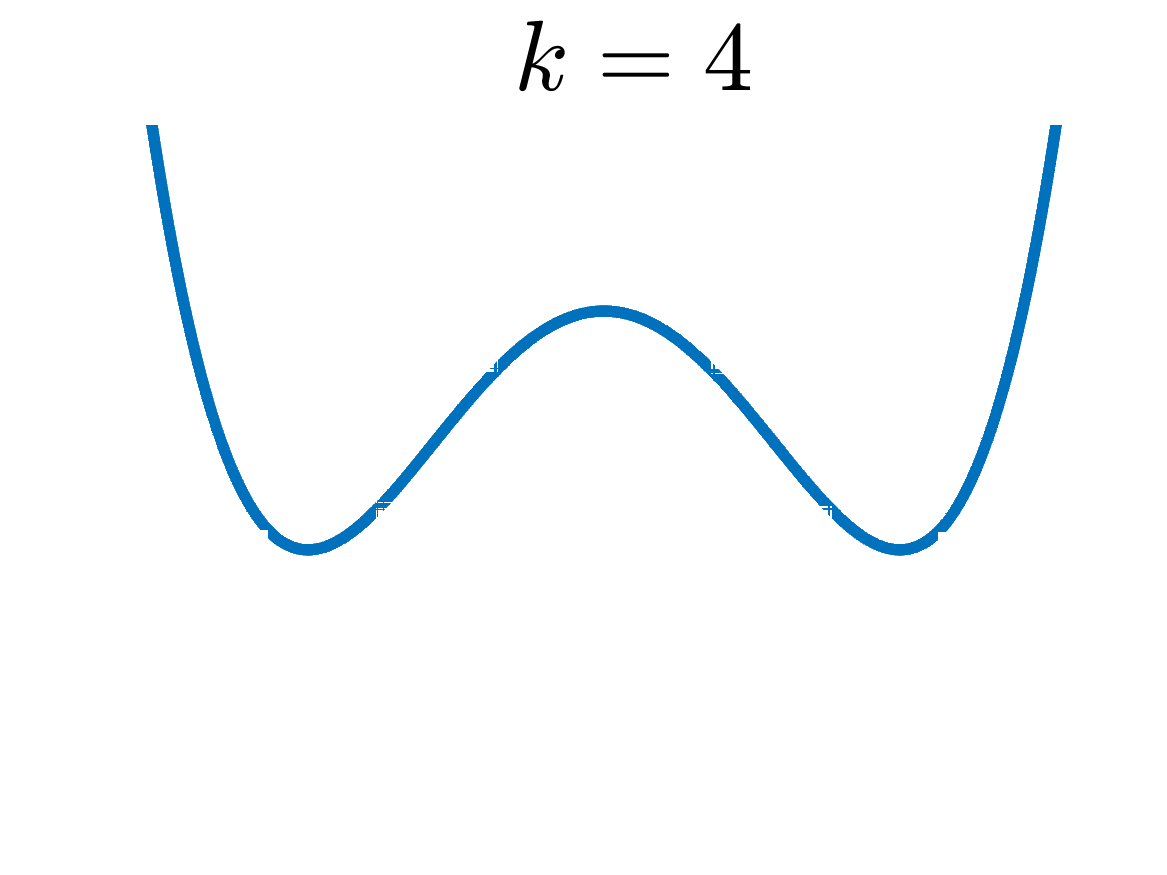
\includegraphics[width =0.18\textwidth]{ProgramsImages/Legendre_Degree_4_1D_k.png} 
	\tabularnewline[-7ex]
	Legendre
	\tabularnewline
\tabularnewline[3ex]
		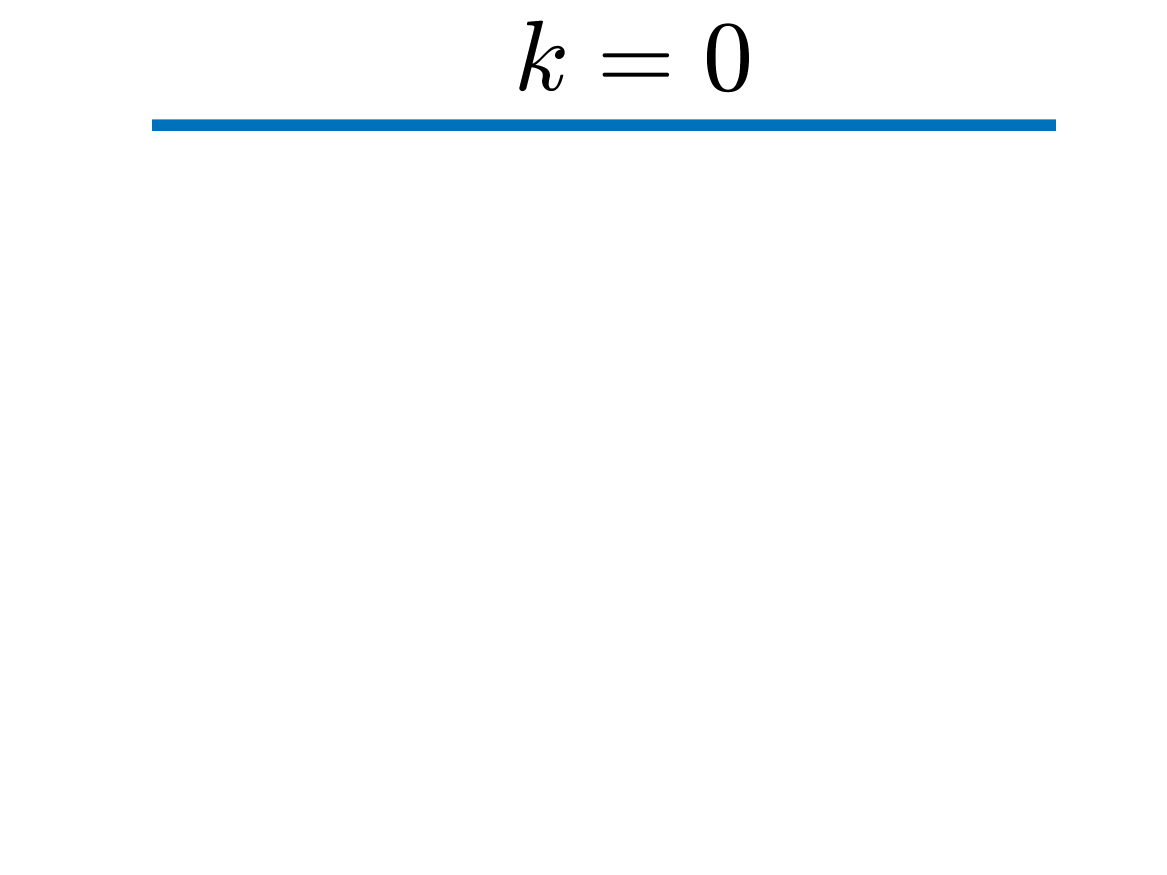
\includegraphics[width =0.18\textwidth]{ProgramsImages/Chebyshev_Degree_0_1D_k.png}  &
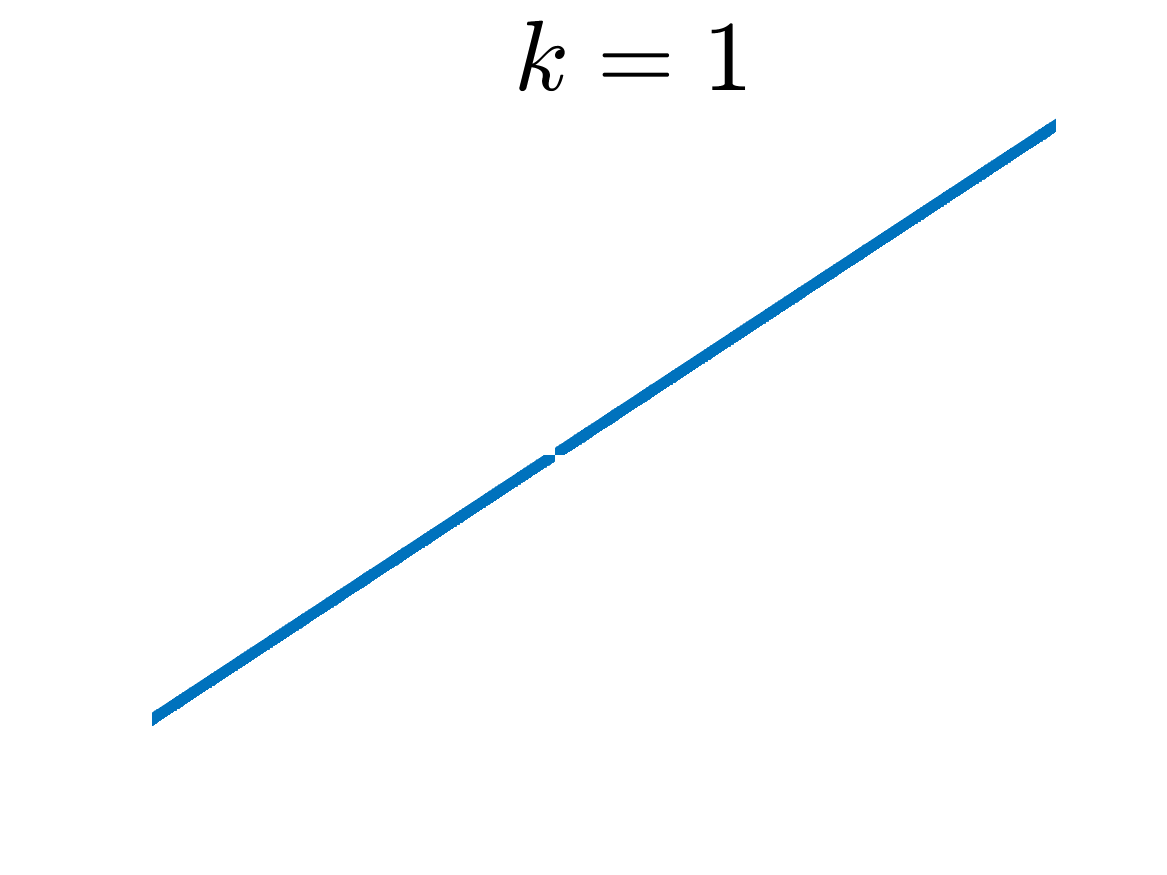
\includegraphics[width =0.18\textwidth]{ProgramsImages/Chebyshev_Degree_1_1D_k.png}  &
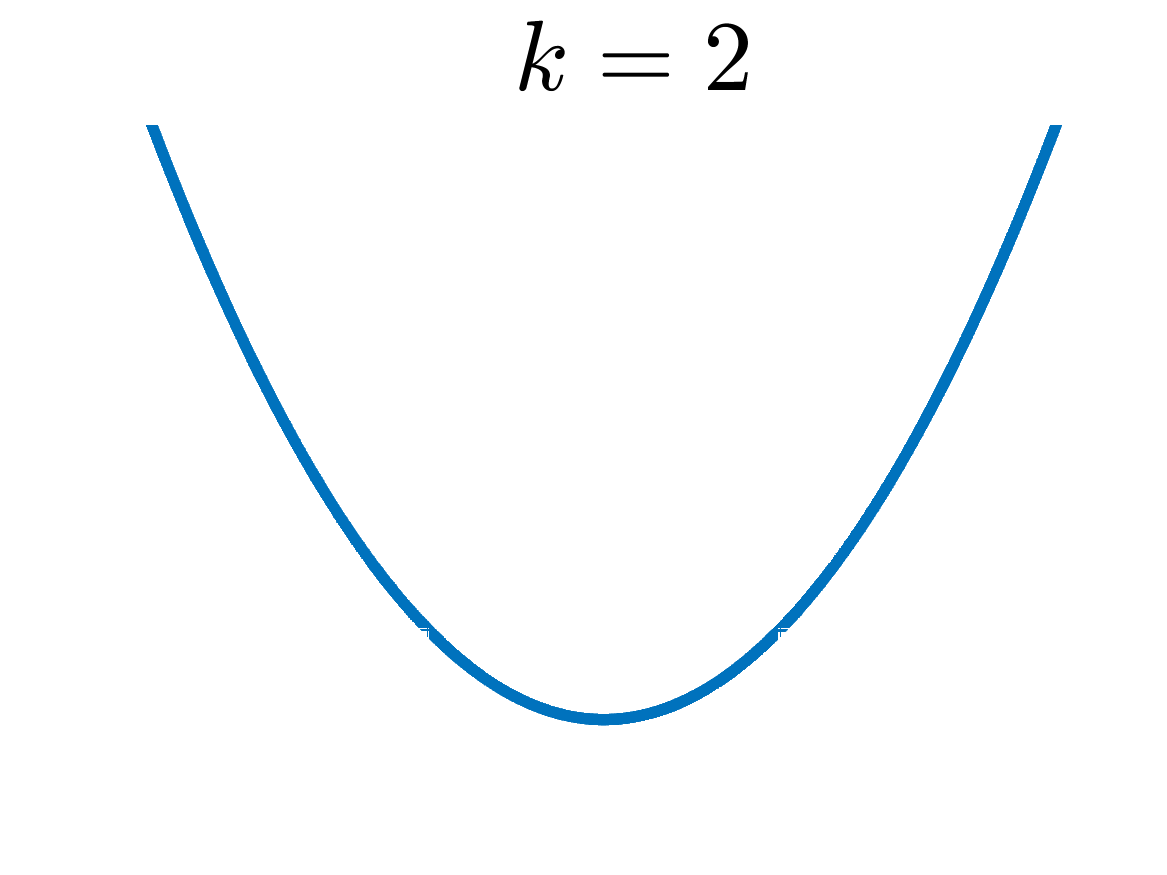
\includegraphics[width =0.18\textwidth]{ProgramsImages/Chebyshev_Degree_2_1D_k.png}  &
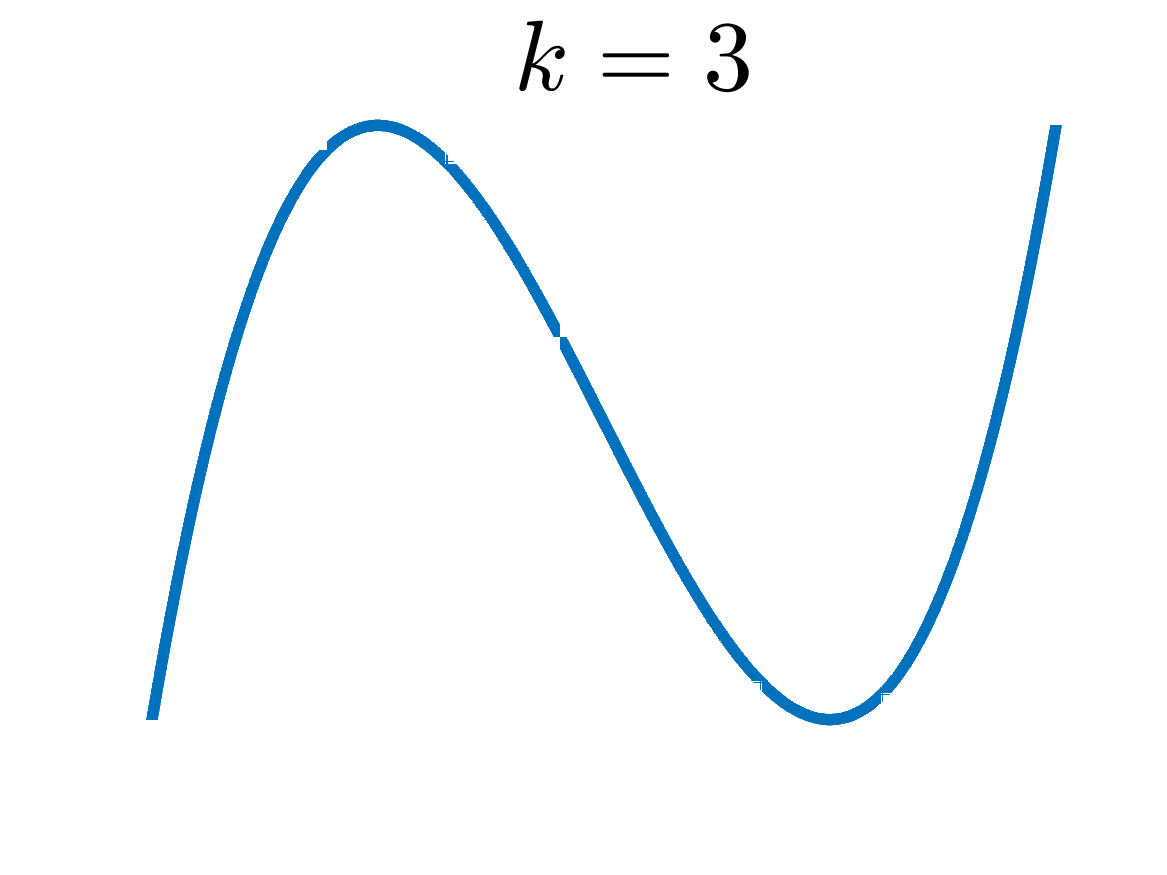
\includegraphics[width =0.18\textwidth]{ProgramsImages/Chebyshev_Degree_3_1D_k.png}  &
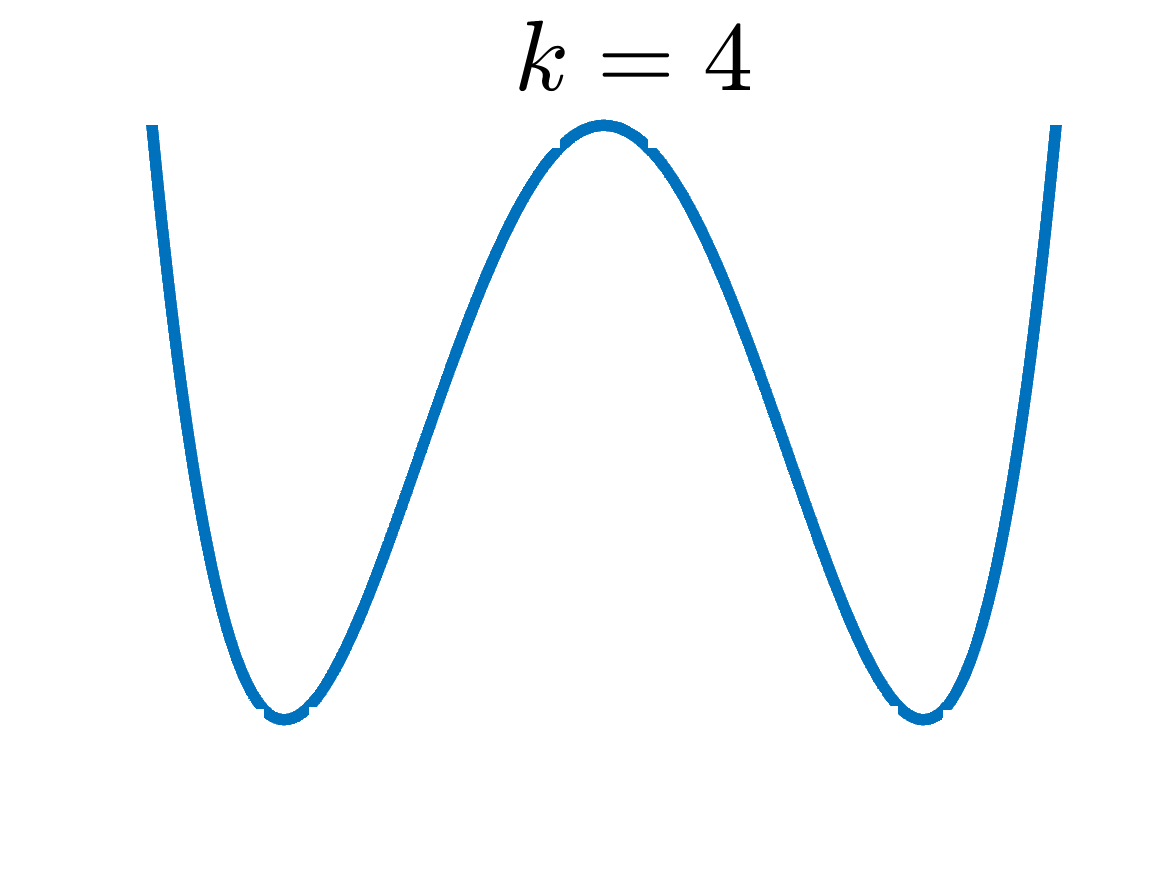
\includegraphics[width =0.18\textwidth]{ProgramsImages/Chebyshev_Degree_4_1D_k.png} 
\tabularnewline[-7ex]
Chebyshev
\tabularnewline
\tabularnewline[3ex]
		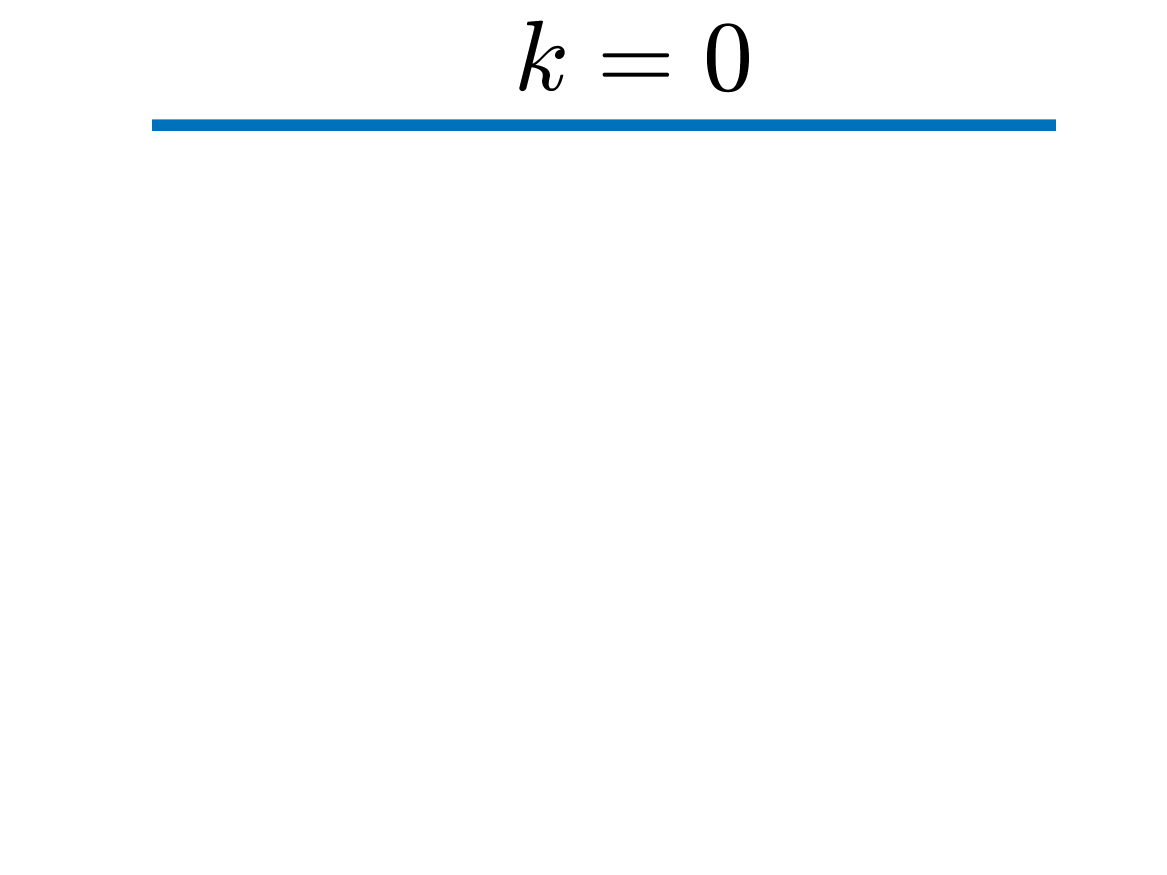
\includegraphics[width =0.18\textwidth]{ProgramsImages/Chebyshev_Degree_0_1D_k.png}  &
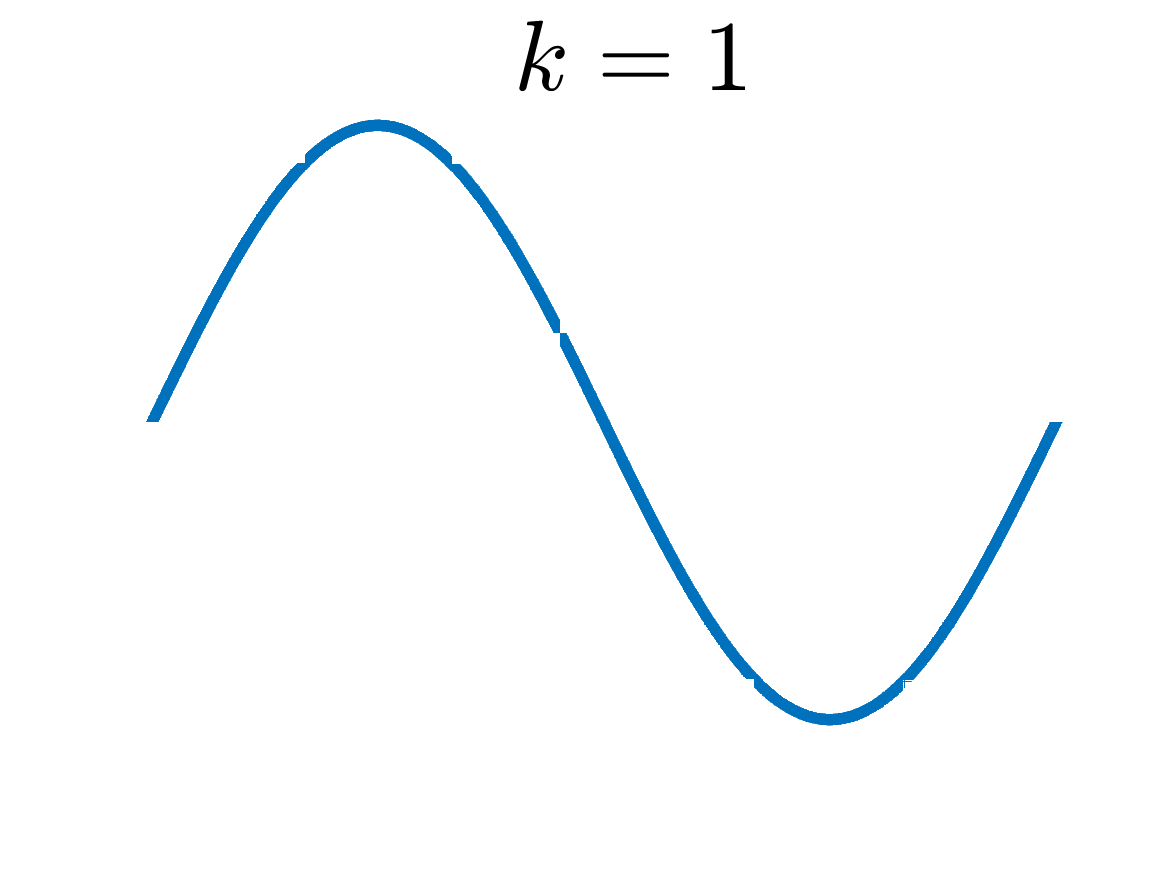
\includegraphics[width =0.18\textwidth]{ProgramsImages/CosineSine_Degree_1_1D_k.png}  &
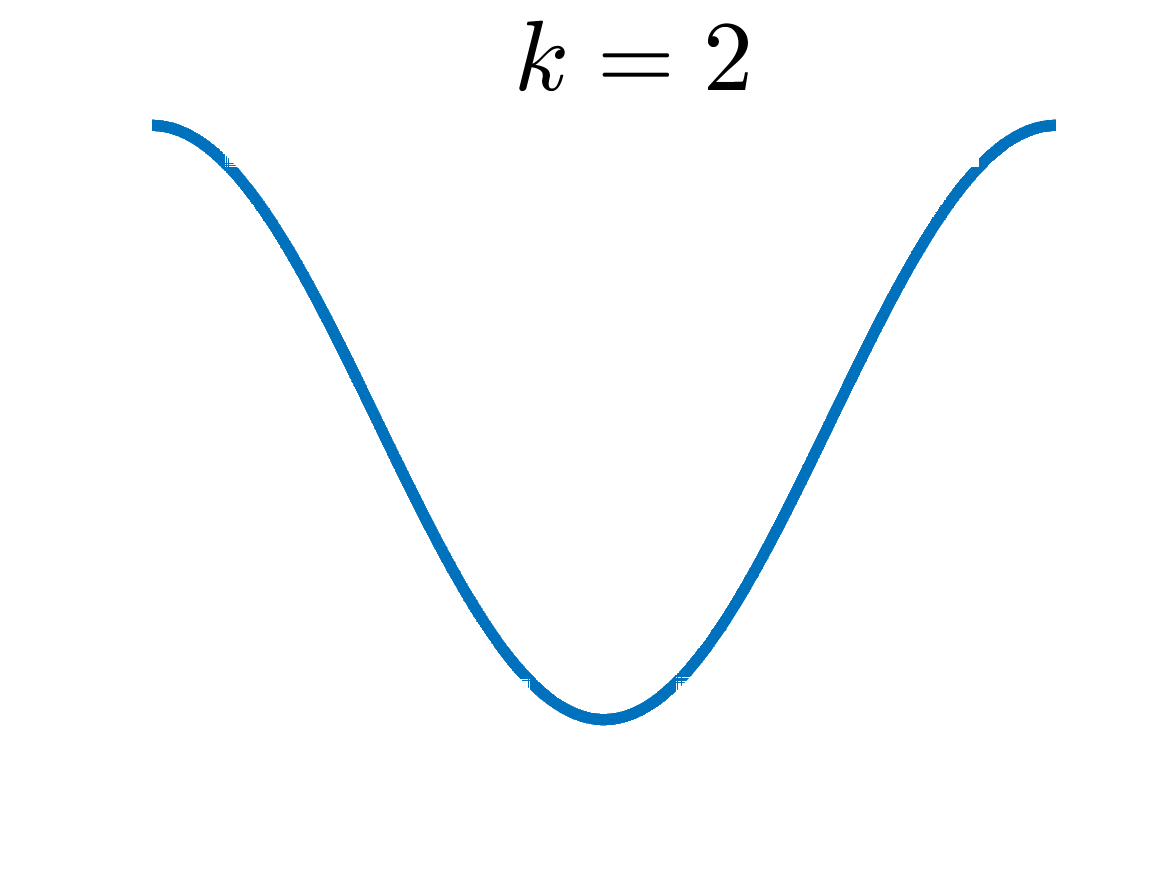
\includegraphics[width =0.18\textwidth]{ProgramsImages/CosineSine_Degree_2_1D_k.png}  &
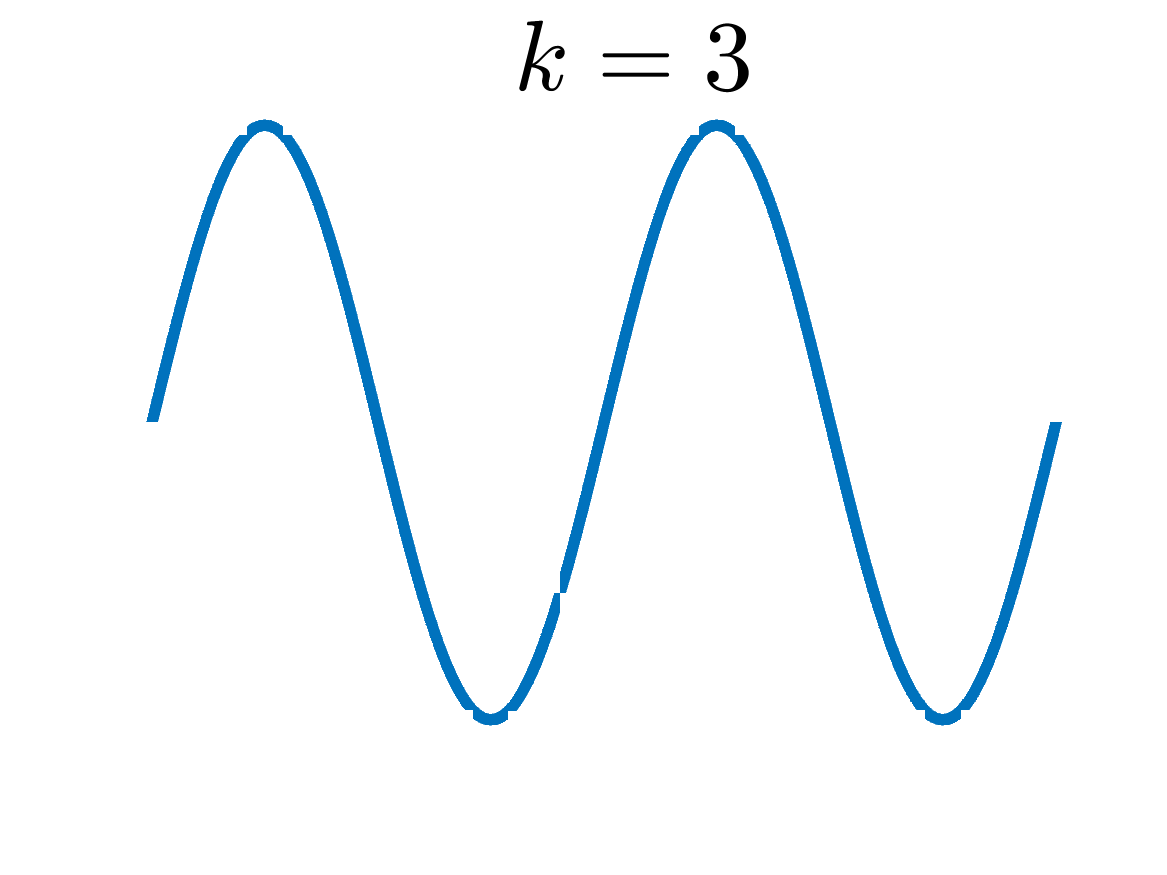
\includegraphics[width =0.18\textwidth]{ProgramsImages/CosineSine_Degree_3_1D_k.png}  &
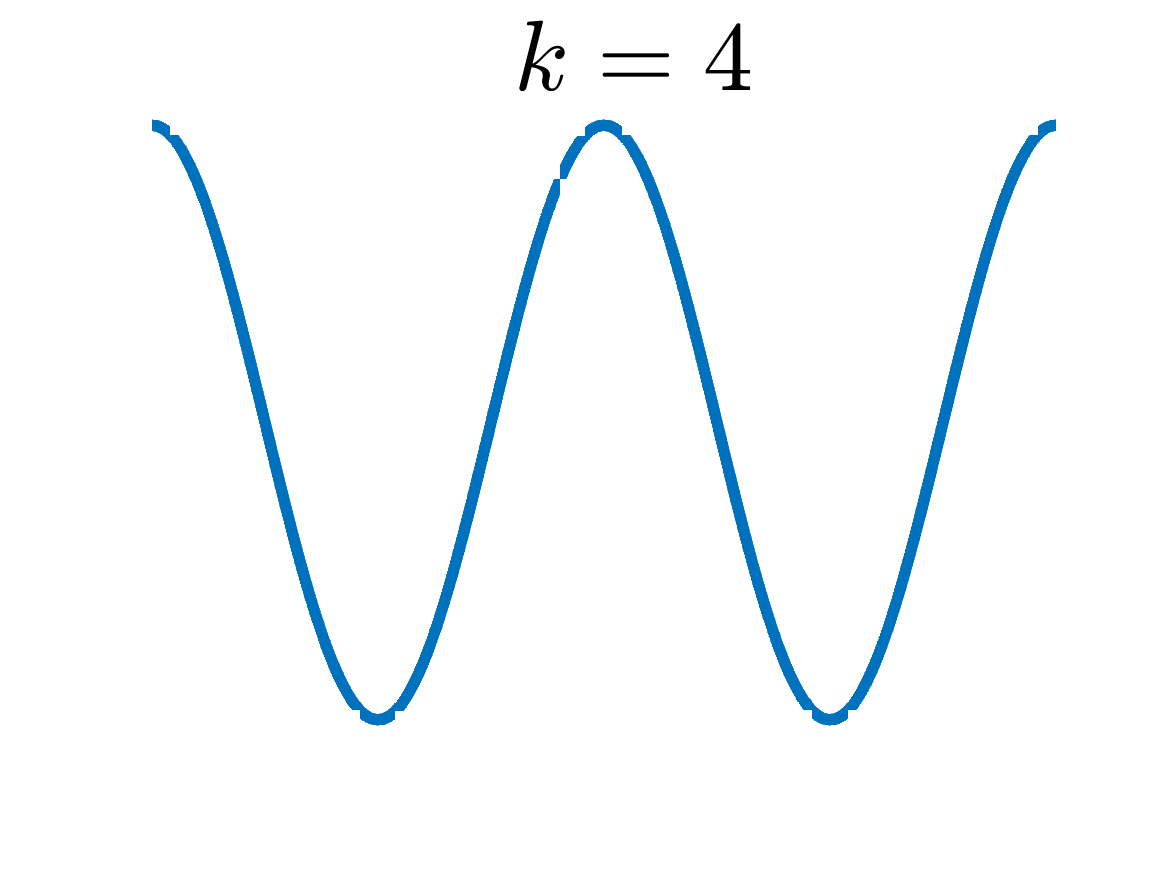
\includegraphics[width =0.18\textwidth]{ProgramsImages/CosineSine_Degree_4_1D_k.png} 
\tabularnewline[-7ex]
Sine and Cosine \tabularnewline
	\end{tabular}
\end{frame}

\againframe<2->{smoothness}

%%%%%%%%%%%%%%%%%%%%%%%%%%%%%%%%%%%%%%%%%%%%%%%%%%%%%%%%%%%%%%%%%%%%
\section{Tractability}
%%%%%%%%%%%%%%%%%%%%%%%%%%%%%%%%%%%%%%%%%%%%%%%%%%%%%%%%%%%%%%%%%%%%
\begin{frame}<1>[label = tract]{\only<1-2>{Smoothness Cannot Save You from the Curse of Dimensionality}\only<3->{Coordinate Weights Can Save You\only<4->{, Even with Higher Order Polynomials}}\footfullcite{NovWoz08a}}
\vspace{-3ex}
For \alert{arbitrary $d$}, let $\{u_0 = 1, u_1\only<4->{\alert{, \ldots}}\}$ be used to construct a product basis $\cf$ and $\cg$ \only<1-3>{(multlinear functions)}

\vspace{-6ex}
\begin{gather*}
    \cf := \left \{ f(\vx) 
    = \sum_{\vk \in \only<1-3>{\{0,1\}^d}\only<4->{\alert{\natzero^d}}} \hf(\vk) u_\vk  : \norm[\cf]{f} : = \norm[2]{\left(\frac{\hf(\vk)}{\lambda_\vk} \right)_{\vk \in \only<1-3>{\{0,1\}^d}\only<4->{\alert{\natzero^d}}} } < \infty \right \}, \qquad u_\vk(\vx) := \prod_{\ell = 1}^d u_{k_\ell} (x_\ell)\\
   \cg := \left \{ g = \sum_{\vk \in \only<1-3>{\{0,1\}^d}\only<4->{\alert{\natzero^d}}} \hg(\vk) u_\vk  : \norm[\cg]{g} : = \norm[2]{\bigl(\hg(k) \bigr)_{\vk \in \only<1-3>{\{0,1\}^d}\only<4->{\alert{\natzero^d}}} } < \infty \right \}, \qquad \lambda_\vk := \prod_{\substack{\ell = 1 \\ k_\ell \ne 0}}^d \only<3->{\alert<3>{w_\ell}}\only<1-3>{\alert<1-2>{s}}%
   \only<4->{\alert{s_{k_\ell}}} \only<1-2>{= s^{\norm[0]{\vk}}}\\
   \app(f,n) = \sum_{i=1}^n \hf(\vk_i) u_{\vk_i} , \qquad 
   \lambda_{\vk_1} = 1 \ge \only<1-3>{\only<3>{w_1} s =} \lambda_{\vk_2} \ge \cdots \only<1-2>{\ge s^{d}}, \quad \only<3->{\alert<3>{1=w_1 \ge w_2 \ge \cdots }}
   \uncover<2->{\\
    \alg(f,\varepsilon) 
    = \app(f,n^*)\ \ \& \ \ n^* = \min\{n : \lambda_{\vk_{n+1}} \le \varepsilon/R\} \quad \implies \quad
    \norm[\cg]{f - \alg(f,\varepsilon)} \le \varepsilon \quad \forall f \in \cb_R\\
    \lambda_{\vk_n} = \Order\bigl(n^{-1/p}\only<1-2>{\me^{s^p\alert{d}/p}}%
    \only<3->{\exp\bigl(p^{-1} \textstyle \only<3>{s^p}
    \only<4>{\sum_{k=1}^\infty s^p_k} \sum_{\ell=1}^{\alert{d}} w_\ell^p \bigr)}\bigr) 
    \implies \COST(\cb_R,\varepsilon) = \Order\bigr(R^p\varepsilon^{-p}\only<1-2>{\me^{s^p\alert{d}}}%
    \only<3->{\exp\bigl(\textstyle \only<3>{s^p}
    \only<4>{\sum_{k=1}^\infty s^p_k} \sum_{\ell=1}^{\alert{d}} w_\ell^p \bigr)} \bigl) \quad \forall p \quad \only<1-2>{\alert{\text{exponential growth in $d$}}}
    \only<3->{\\ \hspace{3cm}\alert<3->{\text{cost is independent of $d$ if coordinate% 
    \only<4->{ and smoothness} weights decay quickly}}}
 }
\end{gather*}

\end{frame}


\begin{frame}{Bases for Function Approximation}
\vspace{-3ex}
	\begin{tabular}{>{\centering}m{0.18\textwidth}>{\centering}m{0.18\textwidth}>{\centering}m{0.18\textwidth}>{\centering}m{0.18\textwidth}>{\centering}m{0.18\textwidth}}
		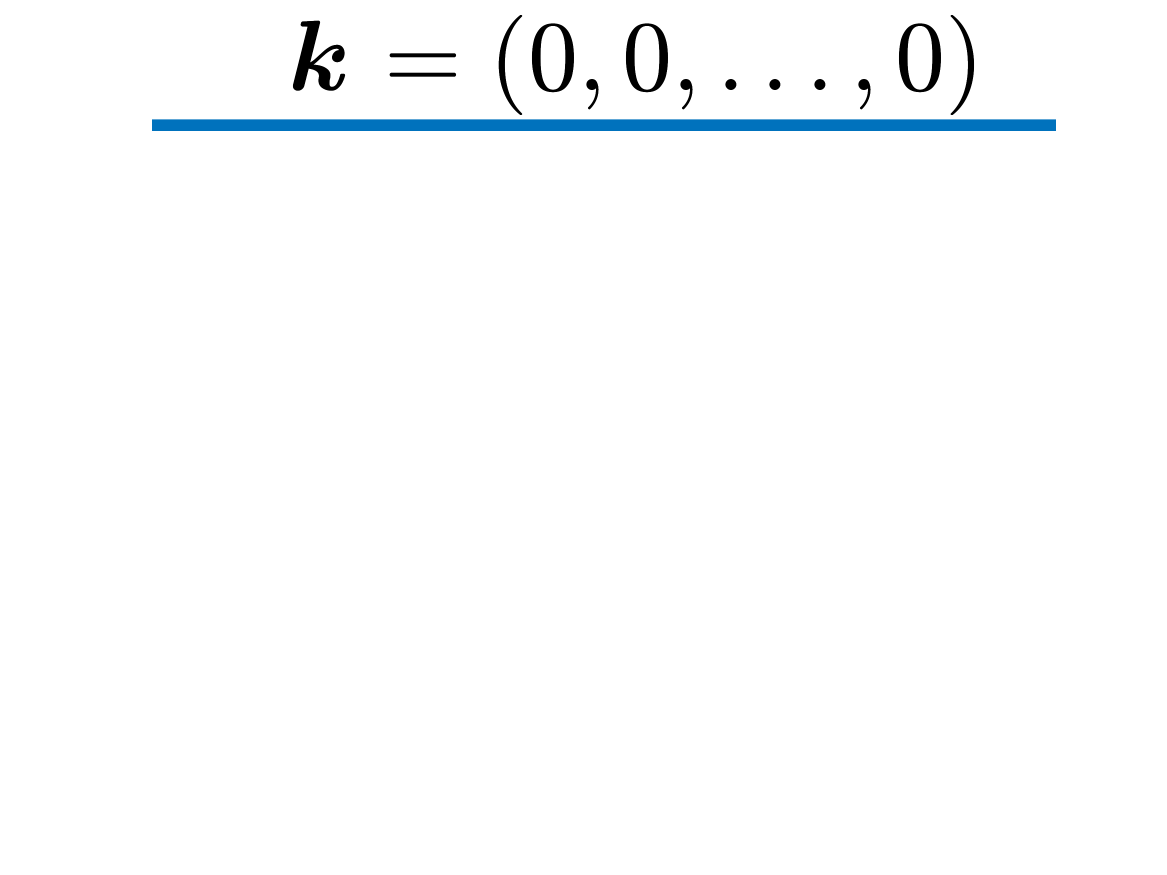
\includegraphics[width =0.18\textwidth]{ProgramsImages/Legendre_Degree_0_k.png}  &
		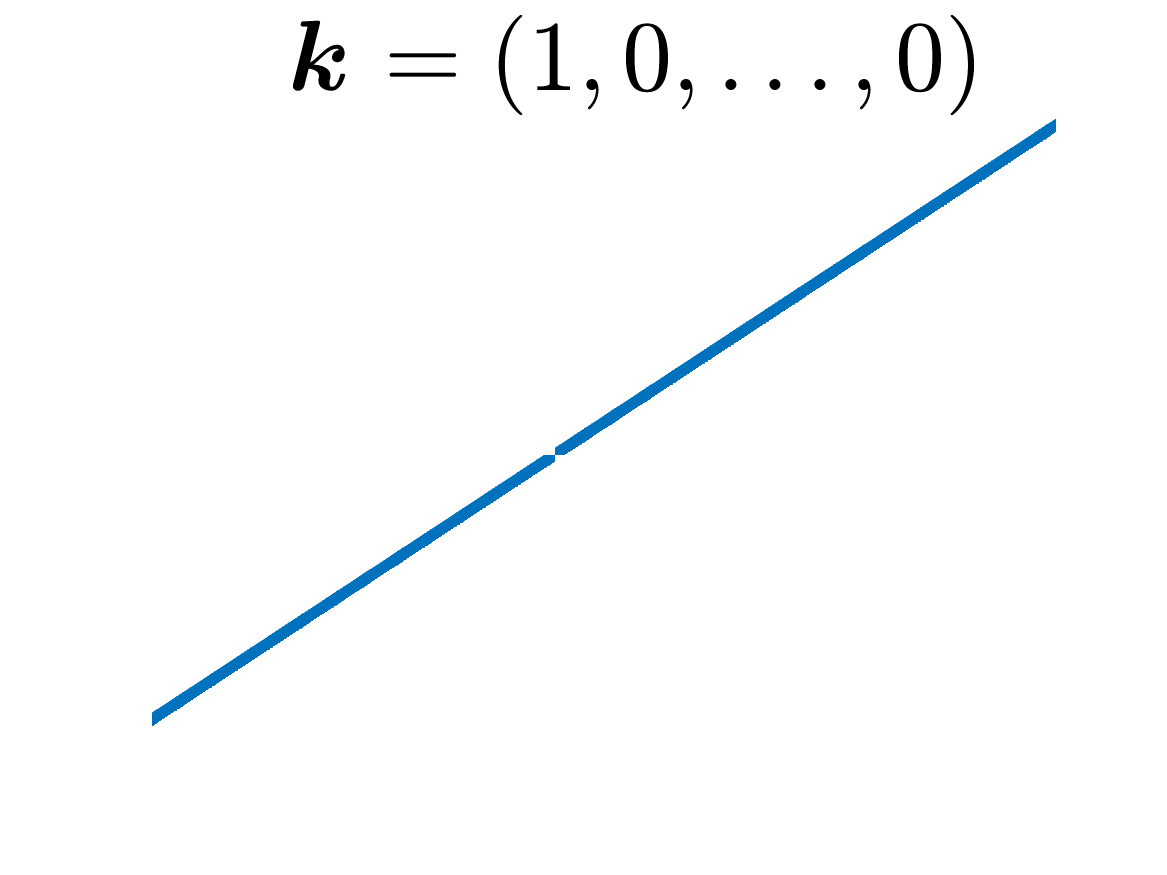
\includegraphics[width =0.18\textwidth]{ProgramsImages/Legendre_Degree_1_k.png}  &
		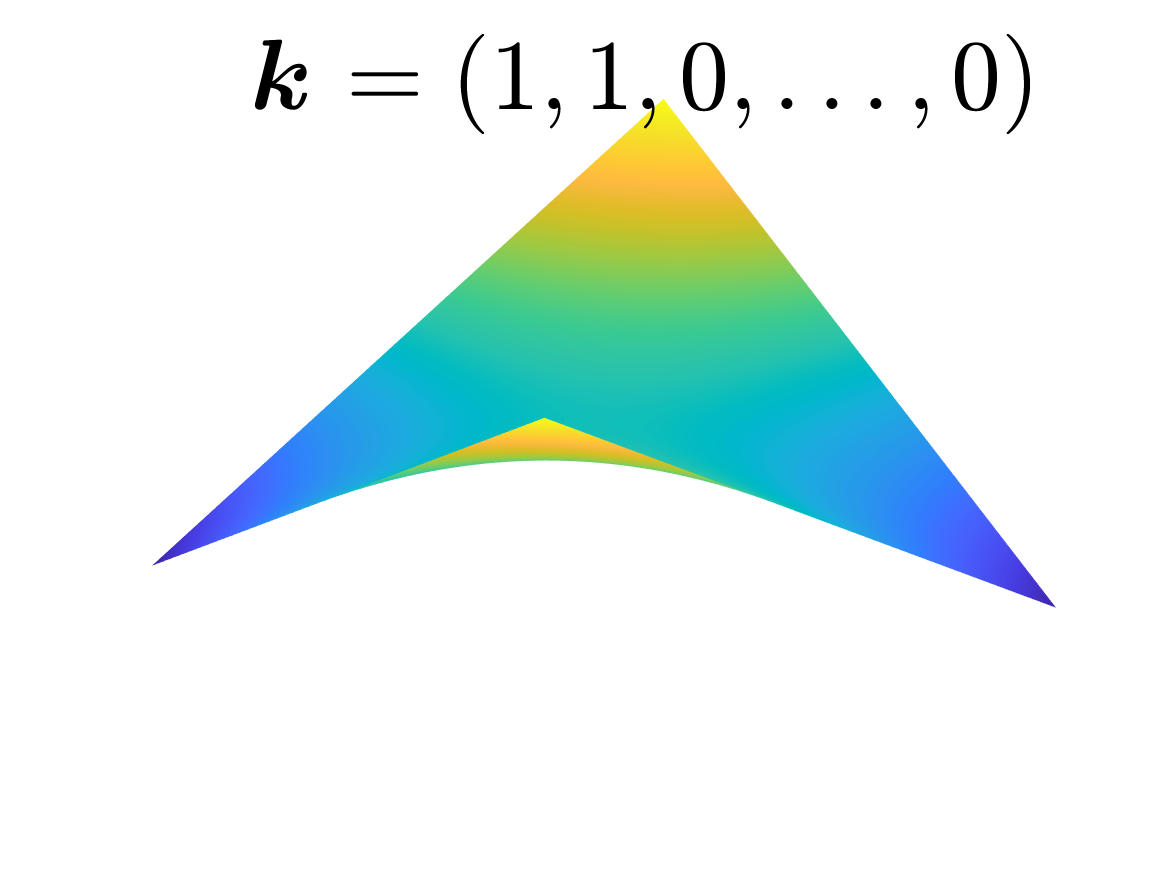
\includegraphics[width =0.18\textwidth]{ProgramsImages/Legendre_Degree_1_1_k.png}
		\tabularnewline[-7ex]
	Legendre
	\tabularnewline
\tabularnewline[3ex]
		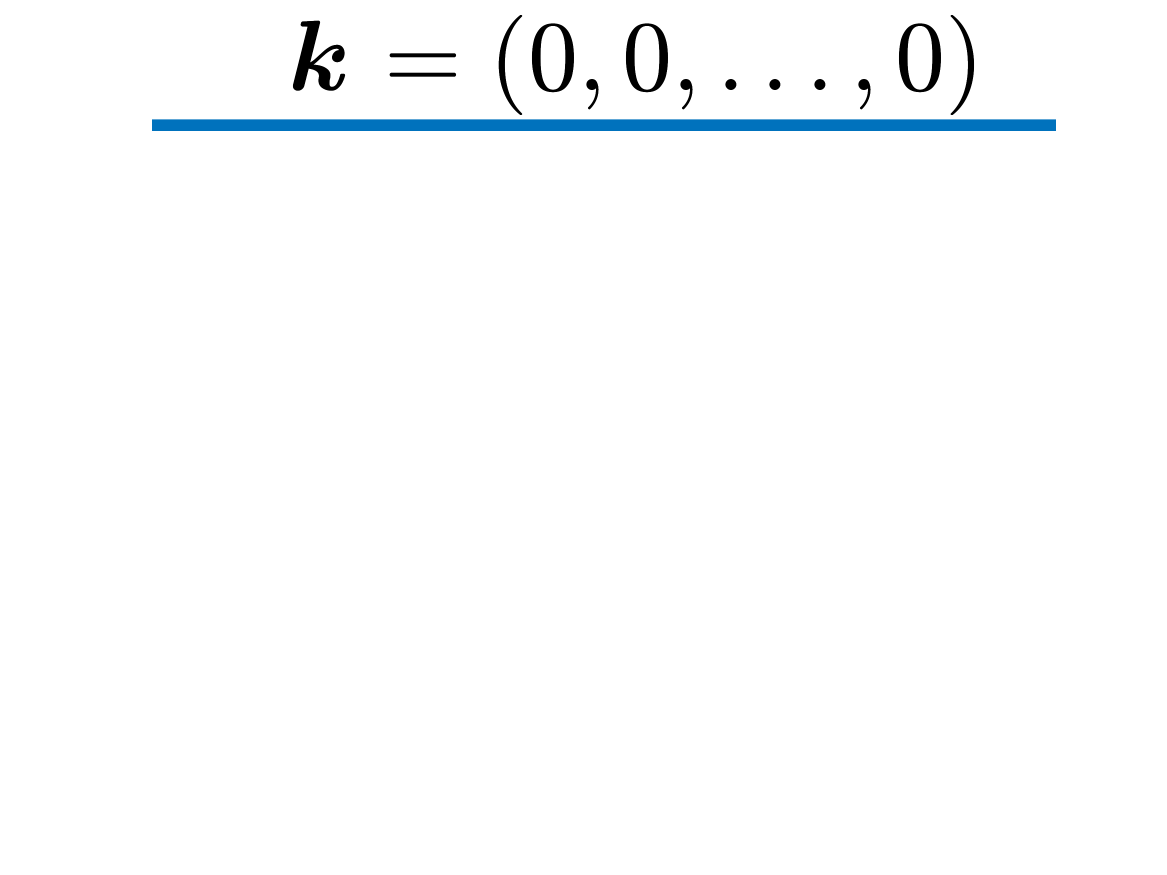
\includegraphics[width =0.18\textwidth]{ProgramsImages/Chebyshev_Degree_0_k.png}  &
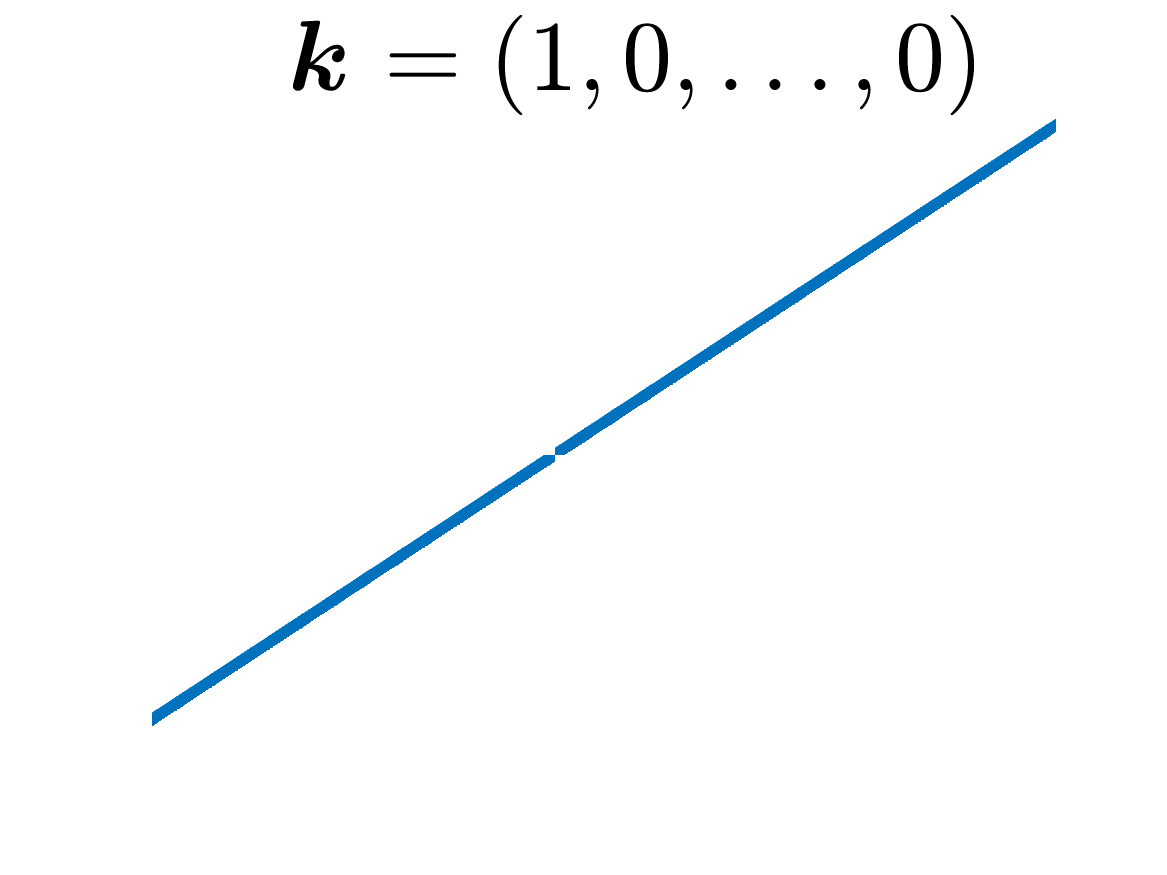
\includegraphics[width =0.18\textwidth]{ProgramsImages/Chebyshev_Degree_1_k.png}  &
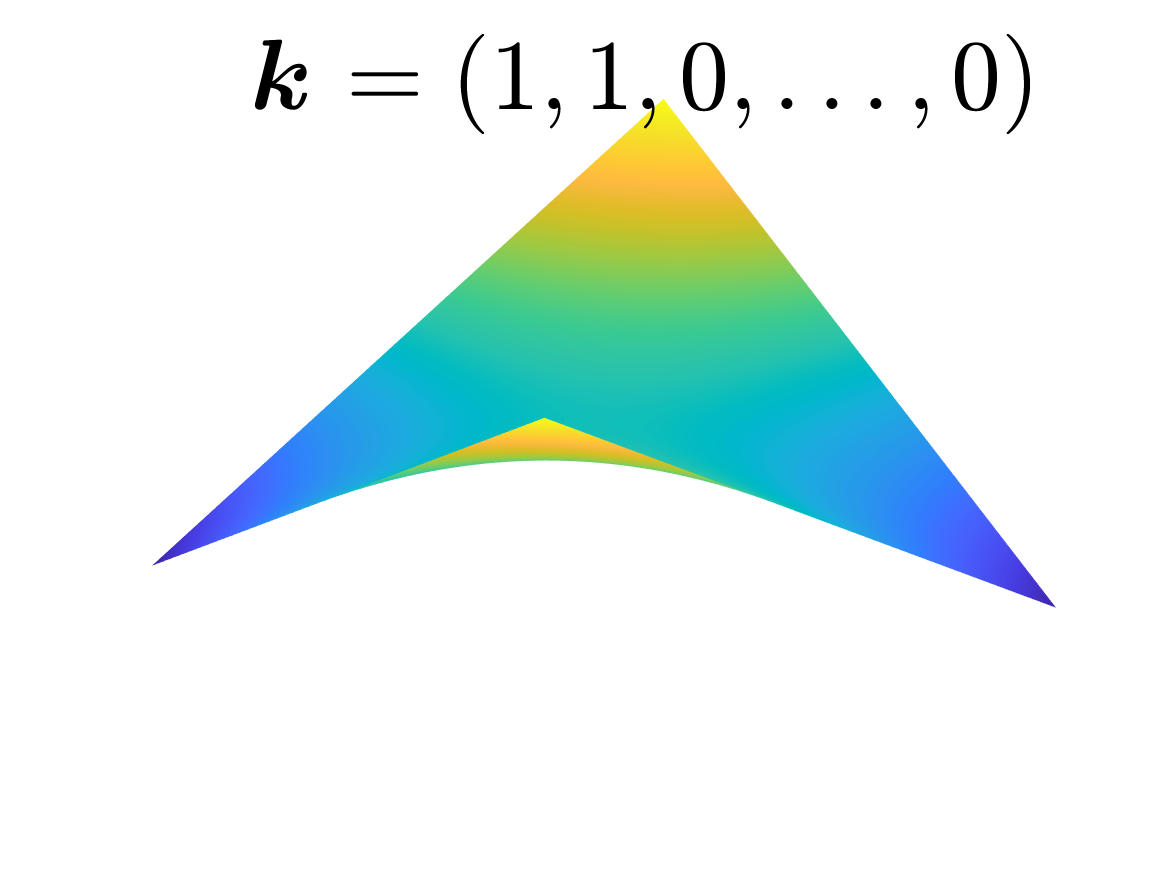
\includegraphics[width =0.18\textwidth]{ProgramsImages/Chebyshev_Degree_1_1_k.png}  
\tabularnewline[-7ex]
Chebyshev
\tabularnewline
\tabularnewline[3ex]
		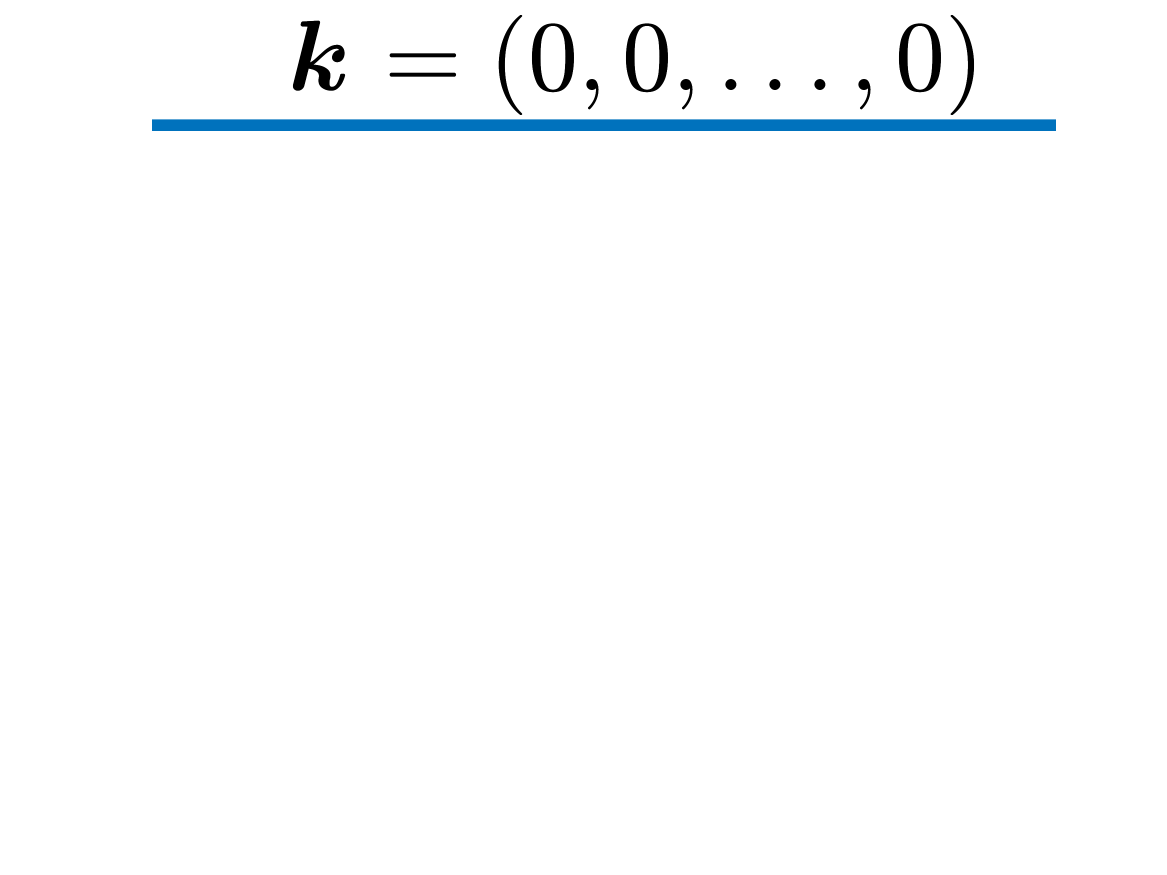
\includegraphics[width =0.18\textwidth]{ProgramsImages/Chebyshev_Degree_0_k.png}  &
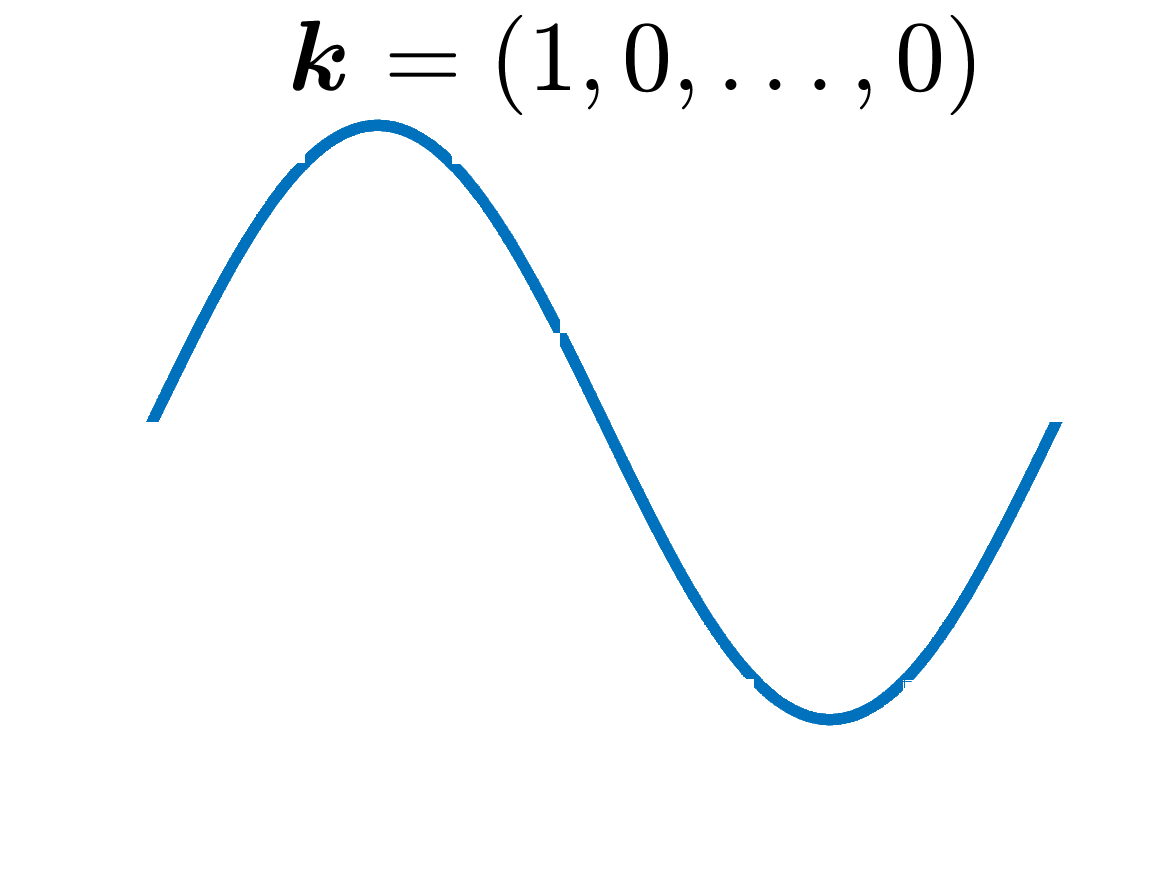
\includegraphics[width =0.18\textwidth]{ProgramsImages/CosineSine_Degree_1_k.png}  &
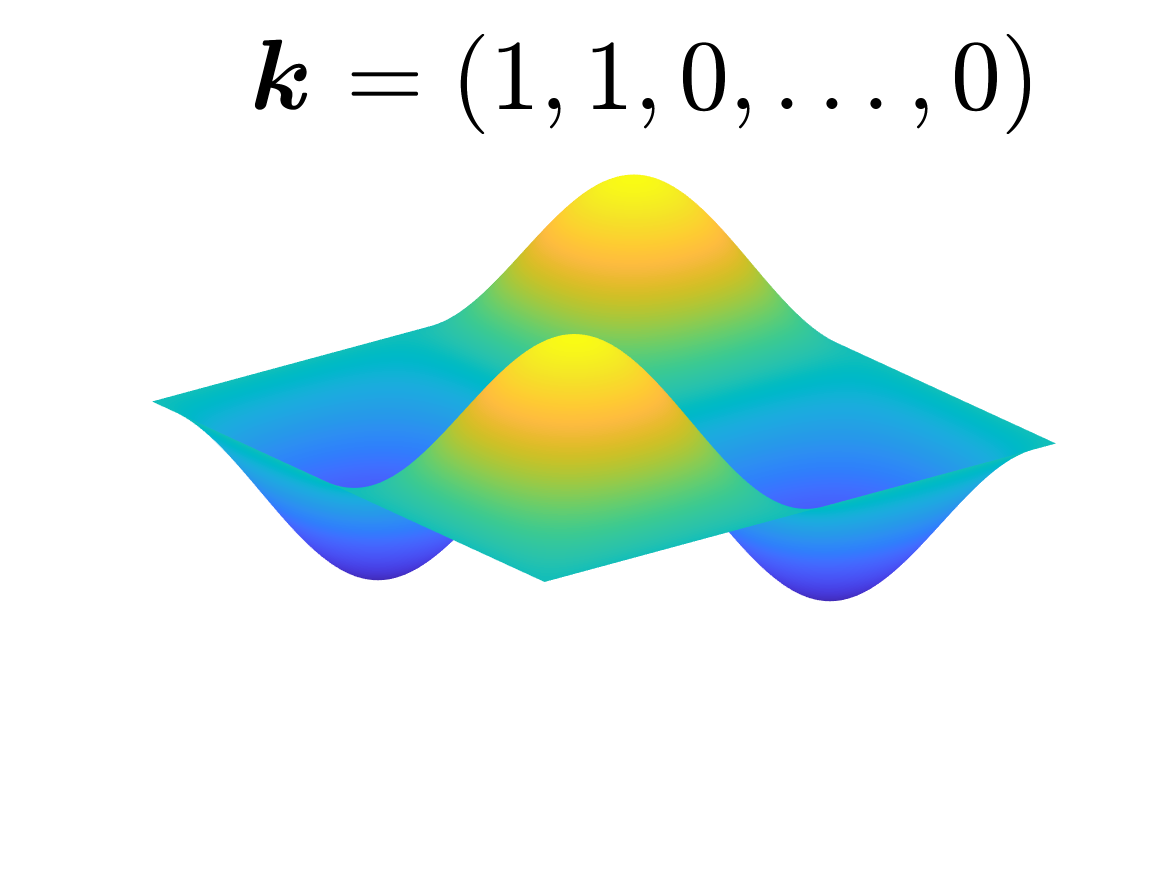
\includegraphics[width =0.18\textwidth]{ProgramsImages/CosineSine_Degree_1_1_k.png}   
\tabularnewline[-7ex]
Sine and Cosine \tabularnewline
	\end{tabular}
\end{frame}


\againframe<2>{tract}

\begin{frame}{Proof that $\lambda_{k_{n+1}} = \Order\bigl(n^{-1/p}\me^{s^p\alert{d}/p}\bigr) \ \forall p > 0$}

\vspace{-6ex}

\begin{align*}
    \lambda_{\vk_{n+1}}^p &\le \frac 1n \bigl( \lambda_{\vk_{1}}^p + \cdots + \lambda_{\vk_{n}}^p \bigr) \qquad \lambda_{\vk_{i}} \text{ are ordered} \\
    \lambda_{\vk_{n+1}} &\le \frac 1{n^{1/p}} \bigl( \lambda_{\vk_{1}}^p + \cdots + \lambda_{\vk_{n}}^p \bigr)^{1/p} \qquad p^{\text{th}} \text{ root} \\
     &\le \frac 1{n^{1/p}} \bigl( \lambda_{\vk_{1}}^p + \cdots + \lambda_{\vk_{2^d}}^p \bigr)^{1/p} \qquad  \text{add the rest in} \\
     &\le \frac 1{n^{1/p}} \bigl( 1 + s^p \bigr)^{\alert{d}/p} \qquad  \text{binomial theorem} \\
     & \le \frac {\me^{s^p\alert{d}/p}}{n^{1/p}} \qquad 1 + x \le \me^x \text{ for } x \ge 0
\end{align*}

There is a similar proof that provides a \alert{lower bound} on $\lambda_{\vk_{n+1}}$
    
\end{frame}

\againframe<3->{tract}

%%%%%%%%%%%%%%%%%%%%%%%%%%%%%%%%%%%%%%%%%%%%%%%%%%%%%%%%%%%%%%%%%%%%
\section{Cones}
%%%%%%%%%%%%%%%%%%%%%%%%%%%%%%%%%%%%%%%%%%%%%%%%%%%%%%%%%%%%%%%%%%%%


\begin{frame}{Look to Cones for Adaptive Algorithms}

\vspace{-4ex}
\alert{Goal:} Construct $\alg$  such that given a \alert{black box} providing information about $f: \Omega \subset \reals^d \to \reals$
\begin{equation*}
    \norm[\cg]{f - \alg(f,\varepsilon)} \le \varepsilon \qquad \forall \varepsilon > 0, \; f \in \ch \subseteq \cf \text{ (Banach space)}
\end{equation*}

\vspace{-5ex}

\begin{itemize}
    \item So far, $\ch = \cb_R$ \smallscoop
    \begin{itemize}
	\setbeamertemplate{itemize items}[triangle]
        \item Hard to know a priori how large $R$ should be for your problem
        \item Computational cost depends on $R$ and $\varepsilon$, but not on $f$ data
    \end{itemize}
    
    \item Choosing $\ch = $ \smallcone makes adaptive algorithms possible\footfullcite{HicEtal17a,KunEtal19a,DinHic20a,RatHic19a}

\end{itemize}
\end{frame}

\begin{frame}[label = Setup]{Adaptive Algorithm for Cone of Inputs Based on Pilot Sample\only<1-3>{\footfullcite{DinEtal20a}}}
	
	\vspace{-7ex}
	
	\begin{align*}
        \cf &:= \left \{ f = \sum_{i=1}^\infty \hf(\vk_i) u_{\vk_i} : \norm[\cf]{f} := \norm[2]{\left(\frac{\bigabs{\hf(\vk_i)}}{\lambda_{\vk_i}} \right)_{i =1}^\infty} \right \} \qquad 
		\begin{minipage}{4.2cm}\raggedright  
		    $\lambda_{\vk_1} \ge \lambda_{\vk_2} \ge \cdots > 0$ \\
		    \alert{$\vlambda$ affects convergence rate \&  \\ tractability}
		\end{minipage}\\
		\cg &: = \biggl \{ g = \sum_{i=1}^\infty \hg(\vk_i) u_{\vk_i} : \norm[\cg]{g} := \bignorm[2]{\hg}\biggr \}, \qquad \app(f,n) = \sum_{i=1}^{n} \hf(\vk_i) u_{\vk_i} \\
	    \uncover<2->{\cc_{d,\vlambda, n_1, A} &: = \Biggl\{ f \in \cf : \norm[\cf]{f} \le A\norm[2]{\biggl ( \frac{\hf(\vk_i) }{\lambda_{\vk_i}} \biggr) _{i=1}^{n_1}} \Biggr\} \qquad 
		\begin{minipage}{6.5cm}\raggedright 
		    \alert{pilot sample bounds the norm of the input \\
		    $A$ is inflation factor, $n_1$ is initial sample size}
		\end{minipage} }
		\end{align*}
		\vspace{-2ex}
\uncover<2->{\begin{equation*}
    \norm[\cg]{f - \app(f,n)} \le \underbrace{\left[ A^2 \norm[2]{\left( \frac{\hf(\vk_i)}{\lambda_{\vk_i}} \right)_{i=1}^{n_1}}^2 -  \norm[2]{\left(\frac{\hf(\vk_i)}{\lambda_{\vk_i}}\right)_{i=1}^n}^2 \right]^{1/2}}_{\text{upper bound on } \norm[\cf]{f - \sum_{i=1}^{n} \hf(\vk_i) u_{\vk_i}}}
    \, 
    \lambda_{\vk_{n+1}} =: \underbrace{\ERRN}_{\alert{\text{data-driven}}}
    \quad 
\end{equation*}
}
    \uncover<3->{\vspace{-2ex}
    \begin{align*}
	\alert<3>{\alg(f,\varepsilon)} & 
	\alert<3>{= \app(f,n^*(f,\varepsilon))} 
	\text{ for } \alert<3>{n^*(f,\varepsilon) = \min \{ n \in \naturals : \ERRN \le \varepsilon\} }
	\\ 
    \only<4->{
    \alert<4>{\COST(\alg,\cc_{d, \vlambda, n_1,A},\varepsilon,R)} 
    & \alert<4>{= \max \bigl \{ n^*(f,\varepsilon) : f \in \cc_{\vlambda, n_1, A} \cap \cb_R = \smallcone \cap \smallscoop \bigr\}} \\
    & \alert<4>{= \min \left \{n \ge n_1 : \lambda_{\vk_{n+1}}
    \le \varepsilon/[(A^2 -1)^{1/2}R] \right \}}
	}
    \end{align*}
    
    \vspace{-4ex}
    \only<4>{$\alg$ is \alert{essentially optimal}; computational cost is \alert{$d$ independent} if $\lambda_{\vk_i}$ decay quickly}
    }

	
\end{frame}

%%%%%%%%%%%%%%%%%%%%%%%%%%%%%%%%%%%%%%%%%%%%%%%%%%%%%%%%%%%%%%%%%%%%
\section{Design}
%%%%%%%%%%%%%%%%%%%%%%%%%%%%%%%%%%%%%%%%%%%%%%%%%%%%%%%%%%%%%%%%%%%%

\begin{frame}{Challenges When Using Function Values as Information}
\vspace{-4ex}
\alert{Goal:} Construct $\alg$  such that given a \alert{black box} providing information about $f: \Omega \subset \reals^d \to \reals$
\begin{equation*}
    \norm[\cg]{f - \alg(f,\varepsilon)} \le \varepsilon \qquad \forall \varepsilon > 0, \; f \in \ch \subseteq \cf \text{ (Banach space)}
\end{equation*}

\vspace{-4ex}

\begin{itemize}
    \item So far, the function information is \alert{series coefficients}
    \begin{itemize}
	\setbeamertemplate{itemize items}[triangle]
        \item $\COST(f,\varepsilon) = \Order\bigl(n^*(f,\varepsilon)\, \$(f)\bigr)$, the best one can hope for
        \item Cost of \alert{constructing the approximation} and determining the \alert{stopping sample size} is essentially the same as getting the data
        \item But using series coefficients is \alert{not so realistic}
    \end{itemize}
    
    \item Developing theory for multivariate function approximation using function values is challenging
    \begin{itemize}
	\setbeamertemplate{itemize items}[triangle]
        \item One must bound the aliasing effects of using interpolation or other means to approximate the coefficients
        
        \item Interpolation, reproducing kernel Hilbert space methods, and kriging typically require $\Order(n^3)$ operations to compute approximation, perhaps more if one is tuning the parameters of the kernels; but there are efforts to speed this up\footfullcite{SchEtal19}
        
        \item Space filling designs such as integration lattices\footfullcite{DicEtal14a}, digital nets\footfullcite{DicPil10a}, and sparse grids\footfullcite{BunGrie04a} are promising
    \end{itemize}
     
\end{itemize}
\end{frame}



%%%%%%%%%%%%%%%%%%%%%%%%%%%%%%%%%%%%%%%%%%%%%%%%%%%%%%%%%%%%%%%%%%%%
\section{Example}
%%%%%%%%%%%%%%%%%%%%%%%%%%%%%%%%%%%%%%%%%%%%%%%%%%%%%%%%%%%%%%%%%%%%

\begin{frame}{Cheng and Sandu Function\footfullcite{DinEtal20a,VirLib17a}}
    \vspace{-9ex}
    \begin{gather*}
        \text{Chebyshev polynomials}, \qquad \text{Coordinate weights } w_\ell \text{ \alert{inferred}}, \qquad
        \text{Smoothness weights } s_k \text{ \alert{inferred}} \\
        \text{\alert{function values} used}
    \end{gather*}
    
    \vspace{-3ex}
    
    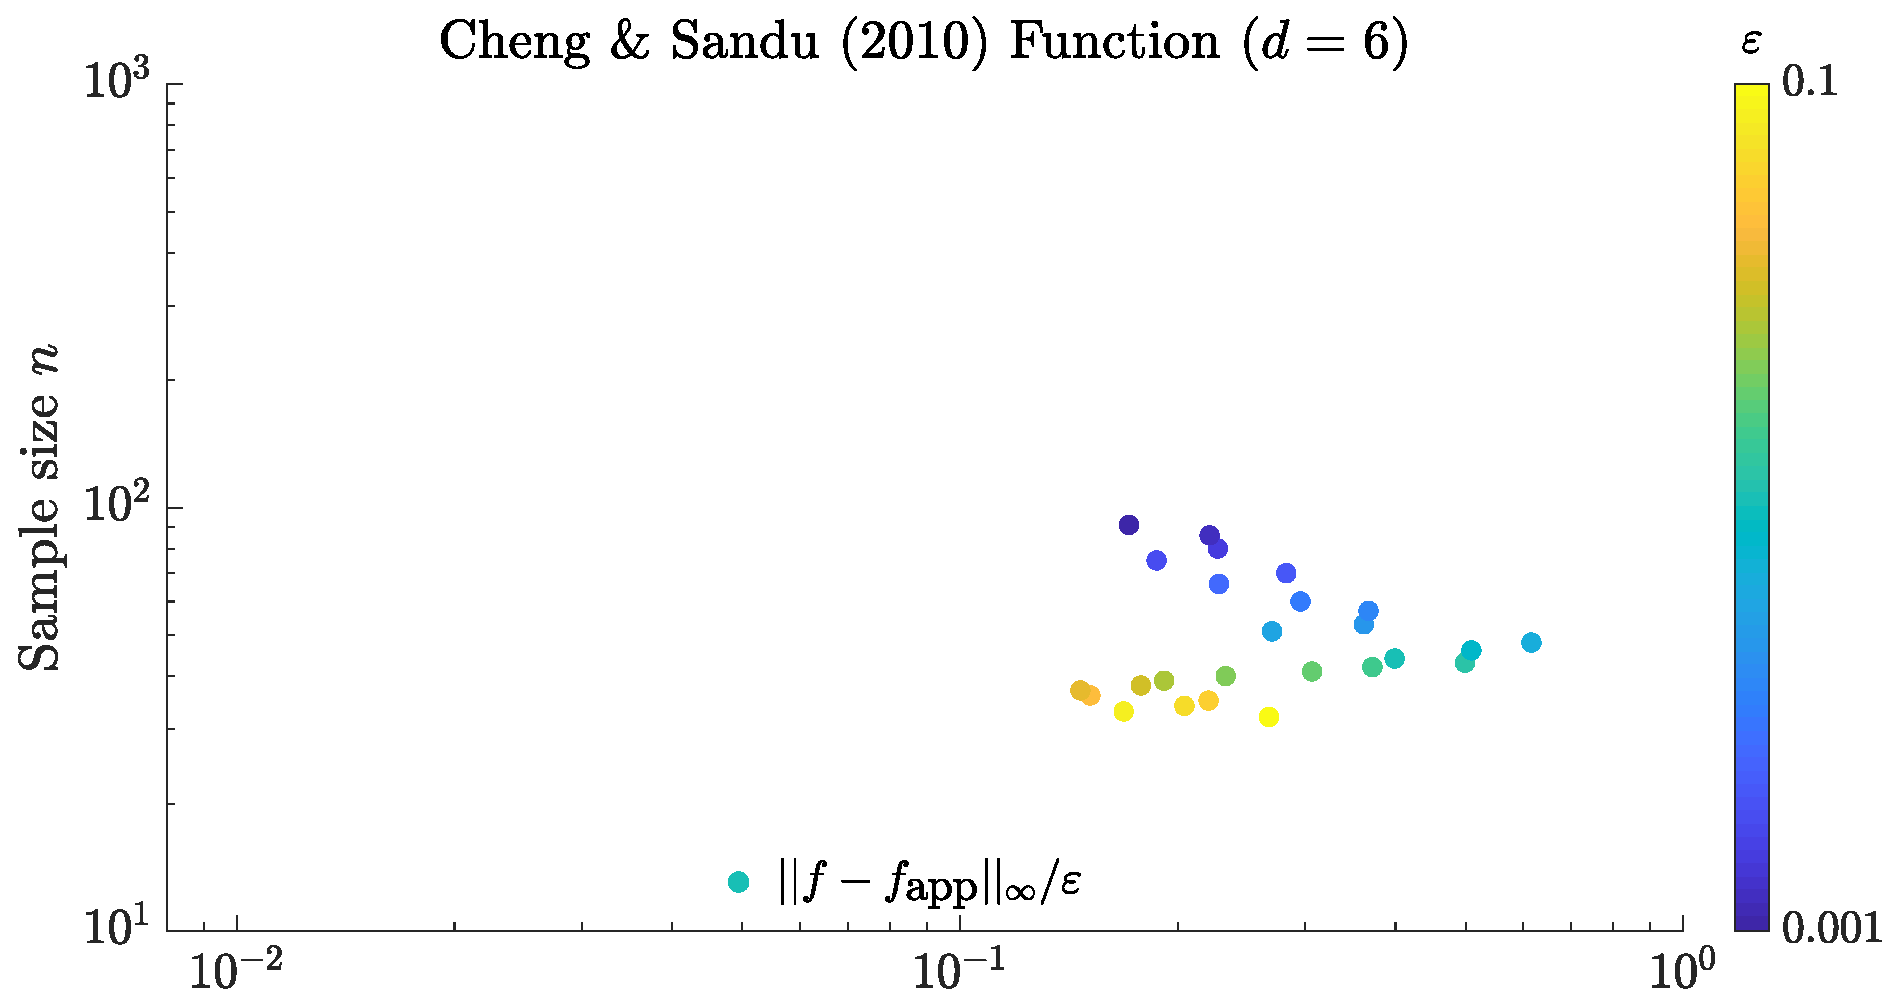
\includegraphics[height = 4.3cm]{ProgramsImages/sim_eval_results_chsan10_d6_sflg0ErrN.eps}
    \qquad 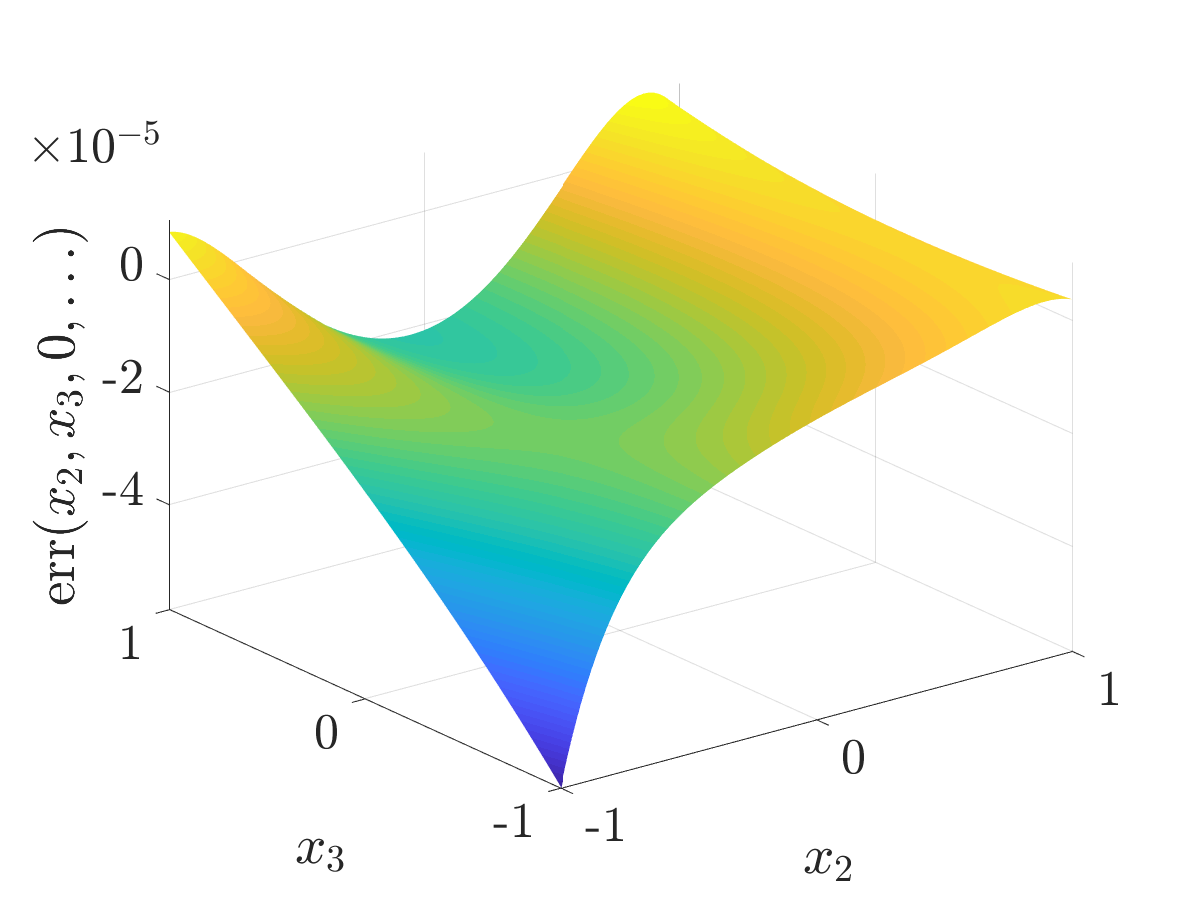
\includegraphics[height = 4.3cm]{ProgramsImages/sim_eval_results_chsan10_d6_sflg0fErr.eps}
\end{frame}


\againframe{high}


\finalthanksnote{These slides are  available at \\  \href{https://speakerdeck.com/fjhickernell/compmath-stat-2019-aug}{\nolinkurl{speakerdeck.com/fjhickernell/compmath-stat-2019-aug}}}


\thankyouframe

\printbibliography





\end{document}

